\chapter{Modular multibody systems in port-Hamiltonian form}\label{ch:fmdPH}

\epigraph{One of my earliest memories of something that caught my attention was of a steam locomotive. I guess mainly because they have so many moving parts that are out in the open. You can watch the valves moving back and forth — the driving rods.}{\textit{Jim Peebles}}

\minitoc

\lettrine{\color{theme}{I}}n this chapter, the pH framework is combined with a floating frame description of the flexible dynamics under large rigid body displacements. Starting from the general equation for the rigid flexible dynamics of a floating body, an equivalent port-Hamiltonian system is found by appropriate selection of the canonical momenta. The flexible behavior is based on the linear elasticity assumption making it possible to include all kinds of linear models. The problem is then written as a coupled system of ordinary and partial differential equations (ODEs and PDEs), extending the general definition of finite-dimensional port-Hamiltonian descriptor systems provided in \cite{mehrmann2019structurepreserving}. The modularity feature of pH systems makes the proposed approach analogous to a substructuring technique: each individual component can be interconnected to the other bodies using standard interconnection of pH systems, as it is done in \cite{macchelli2007link}. This feature allows the use of modeling platforms like {\sc{Simulink}}$^{\tiny{\textregistered}}$ or {\sc{Modelica}}$^{\tiny{\textregistered}}$.  The constraints are imposed on the velocities, leading to a quasi-linear index 2 differential-algebraic port-Hamiltonian system (pHDAE) \cite{steinbrecher2006phd,beattie2018linear}. In the linear case, the algebraic constraints can be eliminated, preserving the overall pH structure, using null space methods \cite{leyendecker2008nullspace}.  As a floating frame formulation is used, model reduction techniques can be employed to lower the computational complexity of the model \cite{chaturantabut2016,egger2018}.  \\


\indent The chapter is organized in the following manner. In Section \ref{sec:class_FMD} the classical equations of a flexible floating body are recalled. Using the properties of the cross product, the equations are recast in a form closer to the pH structure. Section \ref{sec:pH_fd} details the pH formulation of a floating flexible body by introducing the proper canonical momenta. In Section \ref{sec:MB_discr} the PFEM is detailed for the elastodynamics problem. The procedure is easily extended to flexible floating bodies. The particular case of thin planar beams is detailed. Section~\ref{sec:MB_pH} explains how to interconnect models together using classical pH interconnection. 

\section{Flexible dynamics of a floating body}
\label{sec:class_FMD}

\begin{figure}[t]
	\centering
	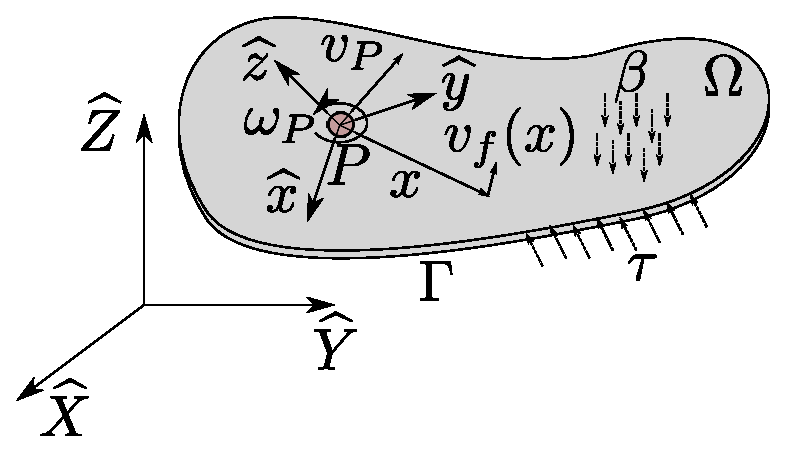
\includegraphics[width=0.6\textwidth]{part_4/pHfmd/floating_body.eps} 
	\caption{Thin floating body undergoing a surface traction $\bm\tau$ and body force density $\bm\beta$}
	\label{fig:float_body}
\end{figure}
The coupled ODE-PDE system representing the motion of a single flexible body is here recalled. Then, by exploiting the properties of the cross product, the system of equations is rephrased to highlight the port-Hamiltonian structure.

\subsection{Classical model}

Consider an open connected set $\Omega \subseteq \mathbb{R}^3$, representing a floating flexible body.  The rigid dynamics is located at point $P$, that is not necessarily the center of mass. The velocity of a generic point is expressed by considering a small flexible displacement superimposed to the rigid motion
\[
\bm{v} = \bm{v}_P + \crmat{\bm{\omega}_P}\bm{x}_f + \bm{v}_f,  \qquad \bm{x}_f := \bm{x}+\bm{u}_f,
\]
where $\bm{x}$ is the position vector of the current point, $\bm{v}_P, \bm{\omega}_P$ are the linear and angular velocities of point $P$  and $\bm{v}_f := \dot{\bm{u}}_f$ is the time derivative of the deformation displacement $\bm{u}_f$ (computed with respect to the body frame). These quantities are evaluated in the body reference frame $\widehat{\bm{x}}, \widehat{\bm{y}}, \widehat{\bm{z}}$ (see Fig. \ref{fig:float_body}). The notation $\crmat{\bm{a}}$ (cross map) denotes the skew-symmetric matrix associated to vector $\bm{a}$ (see Sec. \ref{sec:crossprod}). The model for the classical equations derived using the least action principle can be found in \cite{simeon2006} and \cite[Chapter 4]{simeon2013computational}.

\begin{itemize}
	\item Linear momentum balance:
	\begin{equation}
	\label{eq:ffb_tr_class}
	\begin{split}
	&m ^{i}\ddot{\bm{r}}_P + \bm{R} \crmat{\bm{s}_u}^\top \dot{\bm{\omega}}_P  + \bm{R} \int_{\Omega} \rho \ddot{\bm{u}}_f \d{\Omega} = \\
	&\quad + \bm{R} \left\{ -\crmat{\bm{\omega}_P} \crmat{\bm{\omega}_P} \bm{s}_u -  \int_{\Omega} 2 \rho \crmat{\bm{\omega}_P} \dot{\bm{u}}_f \d{\Omega} +  \int_{\Omega} \bm\beta \d{\Omega} +  \int_{\partial \Omega} \bm\tau \d{\Gamma}  \right\} 
	\end{split}
	\end{equation}
	where $\rho$ is the mass density, $m = \int_{\Omega} \rho \d{\Omega}$ the total mass,  $\bm{s}_u = \int_{\Omega} \rho \bm{x}_f \d{\Omega}$ the static moment. Vector $^{i}{\bm{r}}_P$ is the position of point $P$ in the inertial frame and $\bm{R}$ is the rotation matrix that transforms vectors from the body frame to the inertial frame. Additionally, $\bm\beta$ is a density force and $\bm\tau$ is a surface traction, both expressed in the body reference frame.
	\item Angular momentum balance:
	\begin{equation}
	\label{eq:ffb_rot_class}
	\begin{split}
	\crmat{\bm{s}_u} {\bm{R}^{\top}} \ ^{i}\ddot{\bm{r}}_P + \bm{J}_u \dot{\bm\omega}_P + \int_{\Omega} \rho \crmat{\bm{x}_f} \ddot{\bm{u}}_f \d{\Omega} + \crmat{\bm{\omega}_P} \bm{J}_u \bm{\omega}_P = \\ 
	- \int_{\Omega} 2\rho \crmat{\bm{x}_f} \crmat{\bm\omega_P} \dot{\bm{u}}_f \d{\Omega} + \int_{\Omega}\crmat{\bm{x}_f} \bm\beta \d{\Omega} + \int_{\partial \Omega}\crmat{\bm{x}_f} \bm\tau \d{\Gamma} \\
	\end{split}
	\end{equation}
	where $\bm{J}_u:= \int_{\Omega} \rho \crmat{\bm{x}_f}^\top\crmat{\bm{x}_f} \d{\Omega}= - \int_{\Omega} \rho \crmat{\bm{x}_f}\crmat{\bm{x}_f} \d{\Omega}$ is the inertia matrix.
	\item Flexibility PDE:
	\begin{equation}
	\label{eq:ffb_flex_class}
	\rho  {\bm{R}^{\top}} \ ^{i}\ddot{\bm{r}}_P + \rho (\crmat{\dot{\bm\omega}_P} + \crmat{\bm{\omega}_P}\crmat{\bm{\omega}_P})\bm{x}_f + \rho (2 \crmat{\bm{\omega}_P} \dot{\bm{u}}_f + \ddot{\bm{u}}_f) = \Div{\bm\Sigma} + \bm\beta,
	\end{equation}
	Variable $\bm\Sigma$ is the Cauchy stress tensor. From linear elasticity theory the infinitesimal strain is given by $\bm\varepsilon = \Grad(\bm{u}_f)$. The constitutive equation is expressed as $\bm\Sigma =  \bm{\mathcal{D}} \bm\varepsilon$, where $ \bm{\mathcal{D}}$ is the stiffness tensor (cf. Eq. \eqref{eq:stiff3D}). This PDE requires the specifications of boundary conditions.
	\begin{equation}
	\label{eq:bc_Elas_MB}
	\begin{aligned}
	\bm\Sigma \cdot \bm{n}|_{\Gamma_N} &= \bm\tau|_{\Gamma_N}, \quad \text{$\bm{n}$ is the outward normal,} \\
	\bm{u}_f|_{\Gamma_D} &= \bm{\bar{u}}_f|_{\Gamma_D},
	\end{aligned}
	\end{equation}
	The boundary $\partial \Omega = \overline{\Gamma}_D \cup \overline{\Gamma}_N$ is split into two subsets, one on which the surface traction is imposed ($\Gamma_N$ Neumann condition) and the other where the flexible displacement is known ($\Gamma_D$ Dirichlet condition).
\end{itemize}

\subsection{Towards a port-Hamiltonian formulation}
The gyroscopic terms in Eqs. \eqref{eq:ffb_tr_class}, \eqref{eq:ffb_rot_class}, \eqref{eq:ffb_flex_class} need some manipulations so that the skew-symmetric interconnection operator can be more easily highlighted. The following proposition shows that the classical equations can be rewritten in a more structured form.

\begin{proposition}\label{prop:fmd_pH}
	Denoting by $\bm{v}_f = \dot{\bm{u}}_f$ the derivative of the flexible displacement in the body frame, Equations. \eqref{eq:ffb_tr_class}, \eqref{eq:ffb_rot_class}, \eqref{eq:ffb_flex_class} can be equivalently reformulate as follows
\begin{itemize}
	\item Linear momentum balance:
	\begin{equation}
	\label{eq:ffb_tr_pH}
	\begin{split}
	m\dot{\bm{v}}_P + \crmat{\bm{s}_u}^\top \dot{\bm{\omega}}_P +   \int_{\Omega} \rho \dot{\bm{v}}_f \d{\Omega}  = \\
	\crmat{m {\bm{v}_P} + {\crmat{\bm{s}_u}^\top \bm\omega_P} +2 \int_{\Omega} \rho {\bm{v}_f} \d{\Omega}} \bm\omega_P +  \int_{\Omega} \bm\beta \d{\Omega} + \int_{\partial \Omega} \bm\tau \d{\Gamma}.
	\end{split}
	\end{equation}
	\item Angular momentum balance:
	\begin{equation}
	\label{eq:ffb_rot_pH}
	\begin{split}
	\crmat{\bm{s}_u} \dot{\bm{v}}_P  + \bm{J}_u \dot{\bm\omega}_P + \int_{\Omega} \rho \crmat{\bm{x}_f} \dot{\bm{v}}_f \d{\Omega} = \\
	\crmat{\crmat{\bm{s}_u}^\top \bm\omega_P + 2 \int_{\Omega} \rho {\bm{v}_f} \d{\Omega}} \bm{v}_P + \crmat{\crmat{\bm{s}_u} \bm{v}_P + {\bm{J}_u \bm\omega_P} + 2 \int_{\Omega} \rho \crmat{\bm{x}_f} {\bm{v}}_f \d{\Omega}} \bm\omega_P + 
	\\
	2 \int_{\Omega} \left[\rho \bm{v}_P + \rho \crmat{\bm{x}_f}^\top \, \bm\omega_P\right]_\times \bm{v}_f \d{\Omega} + \int_{\Omega}\crmat{\bm{x}_f} \bm\beta \d{\Omega} + \int_{\partial \Omega}\crmat{\bm{x}_f} \bm{\tau} \d{\Gamma}.
	\end{split}
	\end{equation}
	\item Flexibility PDE:
	\begin{equation}
	\label{eq:ffb_flex_pH}
	\rho \dot{\bm{v}}_P + \rho \crmat{\bm{x}_f}^\top \dot{\bm\omega}_P  + \rho \dot{\bm{v}}_f = \crmat{\rho \bm{v}_P + \rho \crmat{\bm{x}_f}^\top \bm\omega_P + 2 \rho \bm{v}_f} \bm\omega_P + \Div{\bm\Sigma} + \bm\beta.
	\end{equation}
\end{itemize}
\end{proposition} 

\begin{proof}
Equation \eqref{eq:ffb_tr_class} is written in the inertial frame and so it needs to be projected in the body frame. Considering that the position of point $P$, i.e. $^{i}{\bm{r}}_P$, is computed in the inertial frame and $\bm{v}_P$ in the body frame, it holds $^{i}\dot{\bm{r}}_P = \bm{R} \bm{v}_P$. The derivative of this gives
\begin{equation}
\label{eq:acc_rP}
^{i}\ddot{\bm{r}}_P = \bm{R} \left(\dot{\bm{v}}_P + \crmat{\bm{\omega}_P} \bm{v}_P \right)
\end{equation}
If \eqref{eq:acc_rP} is put into \eqref{eq:ffb_tr_class}, \eqref{eq:ffb_rot_class} and \eqref{eq:ffb_flex_class} and pre-multiplying  Eq. \eqref{eq:ffb_tr_class} by $\bm{R}^\top$, it is obtained.
\begin{itemize}
	\item Linear momentum balance:
	\begin{equation}
	\label{eq:ffb_tr_int}
	\begin{split}
	&m (\dot{\bm{v}}_P + \crmat{\bm{\omega}_P} \bm{v}_P) + \crmat{\bm{s}_u}^\top \dot{\bm{\omega}}_P  + \int_{\Omega} \rho \dot{\bm{v}}_f \d{\Omega} = \\
	&\quad - \crmat{\bm{\omega}_P} \crmat{\bm{\omega}_P} \bm{s}_u - \int_{\Omega} 2 \rho \crmat{\bm{\omega}_P} {\bm{v}}_f \d{\Omega} +  \int_{\Omega} \bm\beta \d{\Omega} + \int_{\partial \Omega} \bm\tau \d{\Gamma}.
	\end{split}
	\end{equation}
	\item Angular momentum balance:
	\begin{equation}
	\label{eq:ffb_rot_int}
	\begin{split}
	\crmat{\bm{s}_u} (\dot{\bm{v}}_P + \crmat{\bm{\omega}_P} \bm{v}_P) + \bm{J}_u \dot{\bm\omega}_P + \int_{\Omega} \rho \crmat{\bm{x}_f} \dot{\bm{v}}_f \d{\Omega} + \crmat{\bm{\omega}_P} \bm{J}_u \bm{\omega}_P = \\ 
	- \int_{\Omega} 2\rho \crmat{\bm{x}_f} \crmat{\bm\omega_P} {\bm{v}}_f \d{\Omega} + \int_{\Omega}\crmat{\bm{x}_f} \bm\beta \d{\Omega} + \int_{\partial \Omega}\crmat{\bm{x}_f} \bm\tau \d{\Gamma}. \\
	\end{split}
	\end{equation}
	\item Flexibility PDE:
	\begin{equation}
	\label{eq:ffb_flex_int}
	\rho (\dot{\bm{v}}_P + \crmat{\bm\omega_P} \bm{v}_P) + \rho (\crmat{\dot{\bm\omega}_P} + \crmat{\bm{\omega}_P}\crmat{\bm{\omega}_P})\bm{x}_f + \rho (2 \crmat{\bm{\omega}_P} {\bm{v}}_f + \dot{\bm{v}}_f) = \Div{\bm\Sigma} + \bm\beta,
	\end{equation}
\end{itemize}

Consider now the term $\crmat{\bm{\omega}_P} \crmat{\bm{\omega}_P} \bm{s}_u$, appearing in \eqref{eq:ffb_tr_int}. Using the anticommutativity \eqref{eq:anticom} and the fact that the cross map is skew-symmetric $\crmat{\bm{a}} = -\crmat{\bm{a}}^\top$ one finds
\begin{align*}
-\crmat{\bm{\omega}_P} \crmat{\bm{\omega}_P} \bm{s}_u = \crmat{\crmat{\bm{s}_u}^\top\bm{\omega}_{P}} \bm{\omega}_{P}.
\end{align*}
Eq. \eqref{eq:ffb_tr_int} is then rewritten as
\begin{equation}
\label{eq:ffb_tr_fin}
m\dot{\bm{v}}_P + \crmat{\bm{s}_u}^\top \dot{\bm{\omega}}_P +   \int_{\Omega} \rho \dot{\bm{v}}_f \d{\Omega}  = 
\crmat{m \bm{v}_P + \crmat{\bm{s}_u}^\top \bm\omega_P +2 \int_{\Omega} \rho \bm{v}_f \d{\Omega}} \bm\omega_P +  \int_{\Omega} \bm\beta \d{\Omega} + \int_{\partial \Omega} \bm\tau \d{\Gamma}.
\end{equation}
The terms $\crmat{\bm{s}_u} \crmat{\bm{\omega}_P} \bm{v}_P, \; 2\rho \crmat{\bm{x}_f} \crmat{\bm\omega_P} {\bm{v}}_f$, appearing in \eqref{eq:ffb_rot_int} can be rewritten using the Jacobi identity \eqref{eq:jacobi}
\begin{align}
\crmat{\bm{s}_u} \crmat{\bm{\omega}_P} \bm{v}_P &= - \crmat{\crmat{\bm{s}_u} \bm{v}_P} \bm{\omega}_P - \crmat{\crmat{\bm{s}_u}^\top \bm{\omega}_P} \bm{v}_P, \\
2\rho \crmat{\bm{x}_f} \crmat{\bm\omega_P} {\bm{v}}_f &= - 2\rho \crmat{\crmat{\bm{x}_f} \bm{v}_f}\bm\omega_P - 2\rho \crmat{\crmat{\bm{x}_f}^\top \bm\omega_P} \bm{v}_f
\end{align}
Eq. \eqref{eq:ffb_rot_int} is then rewritten as
\begin{equation}
\label{eq:ffb_rot_fin}
\begin{split}
\crmat{\bm{s}_u} \dot{\bm{v}}_P  + \bm{J}_u \dot{\bm\omega}_P + \int_{\Omega} \rho \crmat{\bm{x}_f} \dot{\bm{v}}_f \d{\Omega} = \\
\crmat{\crmat{\bm{s}_u}^\top \bm\omega_P + 2 \int_{\Omega} \rho \bm{v}_f \d{\Omega}} \bm{v}_P + \crmat{\crmat{\bm{s}_u} \bm{v}_P + \bm{J}_u \bm\omega_P + 2 \int_{\Omega} \rho \crmat{\bm{x}_f} {\bm{v}}_f \d{\Omega}} \bm\omega_P + 
\\
2 \int_{\Omega} \crmat{\rho {\bm{v}_P} + \rho {\crmat{\bm{x}_f}^\top \, \bm\omega_P}} \bm{v}_f \d{\Omega} + \int_{\Omega}\crmat{\bm{x}_f} \bm\beta \d{\Omega} + \int_{\partial \Omega}\crmat{\bm{x}_f} \bm{\tau} \d{\Gamma}.
\end{split}
\end{equation}
Notice that the term $2 \crmat{\bm{v}_f}\bm{v}_P + 2 \crmat{\bm{v}_P}\bm{v}_f = 0$ has been added to the equation. Using again the anticommutativity Eq. \eqref{eq:ffb_flex_int} is expressed as 
\begin{equation}
\label{eq:ffb_flex_fin}
\rho \dot{\bm{v}}_P + \rho \crmat{\bm{x}_f}^\top \dot{\bm\omega}_P  + \rho \dot{\bm{v}}_f = 
\crmat{\rho \bm{v}_P + \rho \crmat{\bm{x}_f}^\top \bm\omega_P + 2 \rho \bm{v}_f} \bm\omega_P + \Div{\bm\Sigma} + \bm\beta.
\end{equation}
Indeed, Eqs. \eqref{eq:ffb_tr_fin}, \eqref{eq:ffb_rot_fin}, \eqref{eq:ffb_flex_fin} are exactly \eqref{eq:ffb_tr_pH}, \eqref{eq:ffb_rot_pH}, \eqref{eq:ffb_flex_pH}.
\end{proof}

By introducing the appropriate momenta, Eqs. \eqref{eq:ffb_tr_pH}, \eqref{eq:ffb_rot_pH}, \eqref{eq:ffb_flex_pH} can be reformulated as a pH system as illustrated in the following section.


\section{Elastic body under large rigid motion as a pH system}
\label{sec:pH_fd}
In this section the flexible dynamics of a floating body is written as a coupled system of ODEs and PDEs in pH form. The final form is a descriptor port-Hamiltonian system that fits and generalizes the framework detailed in \cite{beattie2018linear,mehrmann2019structurepreserving}.  

\subsection{Energies and canonical momenta}
Consider the total energy (Hamiltonian), given by the sum of kinetic and deformation energy:
\begin{equation}
\label{eq:H}
H = H_{\text{kin}} + H_{\text{def}}= \frac{1}{2} \int_{\Omega} \left\{\rho ||\bm{v}_P + \crmat{\bm{\omega}_P} \bm{x}_f + {\bm{v}}_f||^2 + \bm\Sigma \cddot \bm\varepsilon \right\}  \d{\Omega}.
\end{equation}
The inner product $\bm{A} \cddot \bm{B} = \Tr(\bm{A} \bm{B}^T)$ is the tensor contraction.  
The momenta (usually called energy variables in the pH framework) are then computed by derivation of the Hamiltonian. As the variables belong to finite- and infinite-dimensional spaces the derivative is either a classical gradient or a variational derivative:
\begin{equation}
\label{eq:momenta}
\begin{aligned}
\bm{p}_t &:= \diffp{H}{\bm{v}_P} = m \bm{v}_P + \crmat{\bm{s}_u}^\top \, \bm\omega_P + \int_{\Omega} \rho \bm{v}_f \d{\Omega}, \\
\bm{p}_r &:= \diffp{H}{\bm\omega_P} = \crmat{\bm{s}_u} \bm{v}_P + \bm{J}_u \bm\omega_P + \int_{\Omega} \rho \crmat{\bm{x}_f} \bm{v}_f \d{\Omega}, \\
\bm{p}_f &:= \diffd{H}{\bm{v}_f} = \rho \bm{v}_P + \rho \crmat{\bm{x}_f}^\top \, \bm\omega_P + \rho \bm{v}_f, \\
\bm\varepsilon &:= \diffd{H}{\bm\Sigma} = \bm{\mathcal{D}}^{-1} \bm\Sigma= \bm{\mathcal{C}} \bm\Sigma,
\end{aligned}
\end{equation}
where the last derivative is computed with respect to a tensor and $\bm{\mathcal{C}}$ is the compliance tensor \eqref{eq:compl3D}. The relation between energy and co-energy variables is then given by
\begin{equation}
\label{eq:mass_op}
\begin{bmatrix}
\bm{p}_t \\ \bm{p}_r \\ \bm{p}_f \\ \bm\varepsilon \\
\end{bmatrix} = 
\underbrace{\begin{bmatrix}
	m \bm{I}_{3\times 3} & \crmat{\bm{s}_u}^\top & \mathcal{I}_\rho^{\Omega} & 0 \\
	\crmat{\bm{s}_u} & \bm{J}_u & \bm{\mathcal{I}}_{\rho x}^{\Omega} & 0  \\
	(\mathcal{I}_\rho^{\Omega})^* & (\bm{\mathcal{I}}_{\rho x}^{\Omega})^* & \rho & 0  \\
	0 & 0 & 0 & \bm{\mathcal{C}} \\
	\end{bmatrix}}_{{\mathcal{M}}: \; \text{Mass operator}}
\begin{bmatrix}
\bm{v}_P \\ \bm{\omega}_P  \\ \bm{v}_f  \\ \bm\Sigma \\
\end{bmatrix},
\end{equation}
where $\bm{I}_{3\times 3}$ is the identity matrix in $\mathbb{R}^3$. The operators are defined as
\begin{equation*}
\begin{aligned}
\mathcal{I}_\rho^\Omega &:=\int_{\Omega} \rho (\cdot) \d{\Omega}, \\
(\mathcal{I}_\rho^{\Omega})^* &= \rho, \\
\end{aligned} \qquad
\begin{aligned} 
\bm{\mathcal{I}}_{\rho x}^{\Omega} &:= \int_\Omega \rho \crmat{\bm{x}_f} (\cdot) \d{\Omega}, \\
(\bm{\mathcal{I}}_{\rho x}^{\Omega})^* &= \rho \crmat{\bm{x}_f}^\top= -\rho \crmat{\bm{x}_f}. \\
\end{aligned}
\end{equation*}
The mass operator $\mathcal{M}$ is a self-adjoint, positive operator. The kinetic and deformation energy can then be written as
\begin{equation}
H_{\text{kin}} + H_{\text{def}} = \frac{1}{2} \inner[X_{\text{kd}}]{\bm{e}_{\text{kd}}}{{\mathcal{M}} \bm{e}_{\text{kd}}}
\end{equation}
where $\bm{e}_{\text{kd}} = [\bm{v}_P; \, \bm{\omega}_P; \, \bm{v}_f; \bm{\Sigma}]$ and the inner product $\inner[X_{\text{kd}}]{\cdot}{\cdot}$ is taken over the space 
$$ 	X_{\text{kd}} = \mathbb{R}^3 \times \mathbb{R}^3 \times {L}^2(\Omega, \mathbb{R}^3) \times {L}^2(\Omega, \mathbb{R}^{3\times 3}_{\text{sym}})$$ 
Notice that the kinetic energy also depends on the flexible displacement
\[
\diffd{H_{\text{kin}}}{\bm{u}_f} = \crmat{\bm{p}_f} \bm{\omega_{P}}.
\]
This term is responsible for a coupling between the kinematic coordinates and the velocities, as will be clear in the following section. 

\subsection{Port-Hamiltonian formulation}
In order to get a complete formulation, generalized coordinates are required. It is natural to select the following variables:
\begin{itemize}
	\item $^i \bm{r}_P$ the position of point $P$ in the inertial frame of reference;
	\item $\bm{R}$ the direction cosine matrix that transforms vectors from the body frame to the inertial frame (other attitude parametrizations are possible, here the direction cosine matrix is considered for ease of presentation);
	\item $\bm{u}_f$ the flexible displacement;
\end{itemize}

In particular, following \cite{forni2015}, the direction cosine matrix is converted into a vector by concatenating its rows
\begin{equation*}
\bm{R}_{\text{v}} = \text{vec}(\bm{R}^\top) = [\bm{R}_x \; \bm{R}_y \; \bm{R}_z]^\top,
\end{equation*}
where $\bm{R}_{x}, \bm{R}_{y}, \bm{R}_{z}$ are the first, second and third row of matrix $\bm{R}$. Furthermore the corresponding cross map will be given by
\begin{equation*}
\crmat{\bm{R}_{\text{v}}} = 
\begin{bmatrix}
\crmat{\bm{R}_x} \\
\crmat{\bm{R}_y} \\
\crmat{\bm{R}_z} \\
\end{bmatrix}, \qquad 
\crmat{\bm{R}_{\text{v}}} \in \mathbb{R}^{9 \times 3}.
\end{equation*}

The overall port-Hamiltonian formulation, equivalent to Eqs. \eqref{eq:ffb_tr_pH}, \eqref{eq:ffb_tr_pH}, \eqref{eq:ffb_tr_pH}, is then (omitting the external forces and torques)
\begin{equation}
\label{eq:ph_mfd_all}
\setlength{\dashlinegap}{2pt}
\underbrace{
	{\left[ \begin{array}{c:c}
		\bm{I} & \bm{0} \\
		\hdashline
		\bm{0} & \mathcal{M} \\
		\end{array} \right]}
}_{\mathcal{E}}
\diffp{}{t}
\underbrace{
	\begin{pmatrix}
	^i \bm{r}_P \\ \bm{R}_{\text{v}} \\ \bm{u}_f \\\hdashline  \bm{v}_P \\ \bm\omega_P  \\ \bm{v}_f  \\ \bm\Sigma \\
	\end{pmatrix}
}_{\bm{e}} = 
\underbrace{
	{\left[ \begin{array}{ccc:cccc}
		\bm{0} & \bm{0} & \bm{0} &  \bm{R} & \bm{0} & \bm{0} & \bm{0} \\
		\bm{0} & \bm{0} & \bm{0} & \bm{0} & \crmat{\bm{R}_{\text{v}}} & \bm{0} & \bm{0} \\
		\bm{0} & \bm{0} & \bm{0} & \bm{0} & \bm{0} & \bm{I}_{3\times 3} & \bm{0}  \\ 
		\hdashline
		-\bm{R}^\top & \bm{0} & \bm{0} & \bm{0} & \crmat{\widehat{\bm{p}}_t} & \bm{0} & \bm{0} \\
		\bm{0} & -\crmat{\bm{R}_{\text{v}}}^\top & \bm{0} & \crmat{\widehat{\bm{p}}_t} & \crmat{\widehat{\bm{p}}_r} & \bm{\mathcal{I}}_{p_f}^\Omega & \bm{0} \\
		\bm{0} & \bm{0} & -\bm{I}_{3\times 3} & \bm{0} & -(\bm{\mathcal{I}}_{p_f}^\Omega)^* & \bm{0} & \Div \\
		\bm{0} & \bm{0} & \bm{0} & \bm{0} & \bm{0} & \Grad & \bm{0} \\
		\end{array} \right]}
}_{\mathcal{J}}
\underbrace{\begin{pmatrix}
	\partial_{\bm{r}_P}H \\ \partial_{\bm{R}_\text{v}}H \\ \delta_{\bm{u}_f} H \\\hdashline  \bm{v}_P \\ \bm\omega_P  \\ \bm{v}_f  \\ \bm\Sigma \\
	\end{pmatrix}}_{\bm{z}}.
\end{equation} 

Variables $\widehat{\bm{p}}_t, \widehat{\bm{p}}_r$ are defined as
\begin{equation}
\label{eq:mod_momenta}
\begin{aligned}
\widehat{\bm{p}}_t &= \bm{p}_t + \int_{\Omega} \rho \bm{v}_f \d{\Omega}, \\
\widehat{\bm{p}}_r &= \bm{p}_r + \int_{\Omega} \rho \crmat{\bm{x}_f}\bm{v}_f \d{\Omega}. \\
\end{aligned}
\end{equation}
The operator $\bm{\mathcal{I}}_{p_f}^\Omega$ is defined as 
\begin{equation}
\label{eq:mod_momentafl}
\bm{\mathcal{I}}_{p_f}^\Omega := \int_\Omega \left\{2 \crmat{\bm{p}_f} + \rho \crmat{\bm{v}_f} \right\}(\cdot) \d{\Omega}.
\end{equation}
Its  adjoint is given by
\begin{equation*}
(\bm{\mathcal{I}}_{p_f}^\Omega)^* = \left\{2 \crmat{\bm{p}_f}^\top + \rho \crmat{\bm{v}_f}^\top \right\}(\cdot) = - \left\{2 \crmat{\bm{p}_f} + \rho \crmat{\bm{v}_f} \right\}(\cdot).
\end{equation*} 
The coefficient 2 is required to compensate the contribution given by $\delta_{\bm{u}_f} H$ 
\[
-\diffd{H}{\bm{u}_f} - (\bm{\mathcal{I}}_{p_f}^\Omega)^* \bm{\omega}_P = \left[\rho \crmat{\bm{v}_P} + \rho \crmat{\crmat{\bm{x}_f}^\top \bm\omega_P} + 2 \rho \crmat{\bm{v}_f} \right] \bm\omega_P.
\]
The additional terms related to $\rho \bm{v}_f$ are associated to the Coriolis accelerations that affect the deformation field. System \eqref{eq:ph_mfd_all} fits into the framework detailed in \cite{mehrmann2019structurepreserving} and extends it, since a coupled system of ODEs and PDEs is considered. The operator $\bm{\mathcal{J}}$ is skew-symmetric $\bm{\mathcal{J}}_{}^*=-\bm{\mathcal{J}}$ over the Hilbert space
\[
X = \mathbb{R}^3 \times \mathbb{R}^9 \times L^2(\Omega, \mathbb{R}^{3}) \times \mathbb{R}^3 \times \mathbb{R}^3 \times L^2(\Omega, \mathbb{R}^{3}) \times L^2(\Omega, \mathbb{R}^{3\times 3}_{\text{sym}}).
\] 
The dynamics can be rewritten compactly as follows
\begin{equation}
\label{eq:MFD_pHDAE}
\begin{aligned}
\mathcal{E}(\bm{e}) \diffp{\bm{e}}{t} &= \mathcal{J}(\bm{e}) \bm{z}(\bm{e}) + \mathcal{B}_\Omega(\bm{e}) \bm{u}_\Omega + \mathcal{B}_r(\bm{e}) \bm{u}_\partial, \\
\bm{y}_\Omega &= \mathcal{B}_\Omega^*(\bm{e}) \bm{z}(\bm{e}), \\
\bm{y}_r &= \mathcal{B}_r^*(\bm{e}) \bm{z}(\bm{e}), \\
\bm{u}_\partial &= \mathcal{B}_{\partial} \bm{z}(\bm{e}) =  \bm\Sigma \cdot \bm{n}|_{\partial \Omega} = \bm\tau|_{\partial \Omega}, \\
\bm{y}_\partial &= \mathcal{C}_{\partial} \bm{z}(\bm{e}) = \bm{v}_f|_{\partial \Omega},
\end{aligned}
\end{equation}
where $\bm{u}_\Omega = \bm\beta$. Using definitions  \eqref{eq:momenta}, it follows that the Hamiltonian  satisfies 
\begin{equation}
\label{eq:gradH}
\partial_{\bm{e}} H = \bm{\mathcal{E}}^* \bm{z}.
\end{equation}

Adopting the same nomenclature as in \cite{mehrmann2019structurepreserving}, $\bm{e}$ contains the state and $\bm{z}$ contains the effort functions. The operators verify $\mathcal{E} = \mathcal{E}^*, \; \mathcal{J} = -\mathcal{J}^*$. The control operators are expressed as
\begin{align*}
\mathcal{B}_\Omega &= 
\begin{bmatrix}
\bm{0} & \bm{0} & \bm{0} & \mathcal{I}^\Omega & \bm{\mathcal{I}}_{x}^\Omega & \bm{I} & \bm{0}
\end{bmatrix}^\top, \\
\mathcal{B}_r &= 
\begin{bmatrix}
\bm{0} & \bm{0} & \bm{0} & \mathcal{I}^{\Gamma} & \bm{\mathcal{I}}_{x}^{\Gamma} & \bm{0} & \bm{0} \\
\end{bmatrix}^\top,
\end{align*}
where 
\begin{equation*}
\begin{aligned}
\mathcal{I}^\Omega &:=\int_{\Omega} (\cdot) \d{\Omega}, \\
\mathcal{I}^{\Gamma} &:= \int_{\partial \Omega} (\cdot) \d{\Gamma}, \\
\end{aligned} \qquad
\begin{aligned} 
\bm{\mathcal{I}}_{x}^\Omega &:=\int_{\Omega} \crmat{\bm{x}_f} (\cdot) \d{\Omega}, \\
\bm{\mathcal{I}}_{x}^{\Gamma} &:=\int_{\partial \Omega} \crmat{\bm{x}_f} (\cdot) \d{\Gamma}. \\
\end{aligned}
\end{equation*}
The distributed control operator $\mathcal{B}_\Omega$  is compact. The boundary traction force acts on the rigid part through the compact operator $\mathcal{B}_r$. Notice that by definition of adjoint (see Appendix A), the vector $\bm{y}_r$ represents the rigid body velocity at the boundary
\[
\bm{y}_r = (\bm{v}_P + \crmat{\bm{x}_f}^\top \bm{\omega}_P)\vert_{\partial\Omega},
\] 
while $\bm{y}_\Omega$ represents the velocity field in the domain
\[
\bm{y}_\Omega = \bm{v}_P + \crmat{\bm{x}_f}^\top \bm{\omega}_P + \bm{v}_f.
\]
The power balance is naturally embedded in the dynamics 
\begin{equation}
\begin{aligned}
\dot{H}(\bm{e}) &= \langle \partial_{\bm{e}} H, \partial_t {\bm{e}} \rangle_{X} = \langle \mathcal{E}^* \bm{z}, \partial_t {\bm{e}} \rangle_{X}, \\
&= \langle \bm{z}, \mathcal{E} \partial_t {\bm{e}} \rangle_{X}, \quad \text{Adjoint definition}, \\
& = \langle \bm{z}, \mathcal{J}\bm{z} + \mathcal{B}_d(\bm{e}) \bm{u}_d + \mathcal{B}_r(\bm{e}) \bm{u}_\partial \rangle_{X}, \\
& = \langle \bm{y}_\partial,  \bm{u}_\partial \rangle_{L^2(\partial\Omega, \mathbb{R}^3)} + \langle \mathcal{B}_d^* \bm{z}, \bm{u}_d \rangle_{X} + \langle \mathcal{B}_r^* \bm{z}, \bm{u}_\partial \rangle_{X}, \quad \text{I.B.P. on } \mathcal{J}, \\
&= \langle \bm{y}_\partial + \bm{y}_r,  \bm{u}_\partial \rangle_{L^2(\partial\Omega, \mathbb{R}^3)} + \langle \bm{y}_d,  \bm{u}_d \rangle_{L^2(\Omega, \bbR^3)}, \\
\end{aligned}
\end{equation}
where the integration by parts (Stokes theorem) has been used
\begin{equation}
\label{eq:stokes}
\int_{\Omega} \bm\Sigma \cddot \Grad(\bm{v}_f) \d{\Omega} + \int_{\Omega} \Div(\bm\Sigma) \cdot \bm{v}_f \d{\Omega} = \int_{\partial \Omega} (\bm\Sigma \cdot \bm{n}) \cdot \bm{v}_f \d{\Gamma} = \langle \bm{y}_\partial,  \bm{u}_\partial \rangle_{L^2(\partial\Omega, \bbR^3)}.
\end{equation}
The power balance equals the power due to body force and surface traction
\begin{equation}
\begin{aligned}
\dot{H}(\bm{e}) &= \int_{\partial \Omega} \bm{\tau} \cdot \bm{v} \d\Gamma + \int_{\Omega} \bm{\beta} \cdot \bm{v}  \d{\Omega}, \qquad \bm{v} := \bm{v}_P + \crmat{\bm{\omega}_P} \bm{x}_f + {\bm{v}}_f,\\
&= \int_{\partial \Omega} \bm{u}_\partial \cdot \bm{v} \d\Gamma + \int_{\Omega} \bm{u}_\Omega \cdot \bm{v}  \d{\Omega}.
\end{aligned}
\end{equation}

\begin{remark}
	Even if three dimensional elasticity has been taken as example up to this point, other models are easily considered. Beam and plate models are described by appropriate differential operators that replace the $\Div, \Grad$ appearing in \eqref{eq:ph_mfd_all} (see \secref{sec:ph_floatbeam}). {For example in the case of the Kirchhoff plate the three-dimensional divergence is replaced by a planar divergence  for the membrane behavior and a double divergence for the flexural behavior.}
\end{remark}


\begin{remark}
	Conservative forces are easily accounted for by introducing an appropriate potential energy. For example if the gravity force is considered, the corresponding potential energy reads
	\begin{equation*}
	H_{\mathrm{pot}} = \int_{\Omega} \rho g \, ^i r_z \d{\Omega} = \int_{\Omega} \rho g \left[ ^i r_{P, z} +\bm{R}_z \bm{x}_f \right] \d{\Omega},
	\end{equation*}
	where $^i r_z$ is the vertical location of a generic point computed in the inertial frame. The associated co-energy variables are easily obtained
	\begin{align*}
	\partial_{\bm{r}_P}H_{\mathrm{pot}} &= m g \, \widehat{\bm{Z}}, \quad \text{$\widehat{\bm{Z}}$ is the inertial frame vertical direction},\\
	\partial_{\bm{R}_\mathrm{v}}H_{\mathrm{pot}} &= [\bm{0}_{(3, 1)}, \; \bm{0}_{(3, 1)}, \; \int_{\Omega} \rho g \bm{x}_f^\top \d{\Omega}]^\top, \\
	\delta_{\bm{u}_f} H_{\mathrm{pot}} &= \rho g \, \bm{R}_z^\top.
	\end{align*}
	These contributions correspond to the forcing terms due to gravity.
\end{remark}

\begin{remark}
	The linear elasticity hypothesis does not allow including the effect of non-linearities due to large deformations.  However, geometric stiffening could be considered by adding a potential energy associated to centrifugal forces \cite{yigit1988flexural}. 
\end{remark}

\begin{remark}
	If case of vanishing deformations $\bm{u}_f \equiv 0$, the Newton-Euler equations on the Euclidean group $SE(3)$ are retrieved \cite{celledoni2018passivity}
	\begin{equation*}
	\diff{}{t}
	\begin{pmatrix}
	^i{\bm{r}}_P \\
	\bm{R}_{\mathrm{v}} \\
	{\bm{p}}_t \\ 
	{\bm{p}}_r \\
	\end{pmatrix} = 
	\begin{bmatrix}
	\bm{0} & \bm{0} &\bm{R} & \bm{0} \\
	\bm{0} & \bm{0} & \bm{0} & \crmat{\bm{R}_{\mathrm{v}}} \\
	- \bm{R}^\top & \bm{0} & \bm{0} & \crmat{\bm{p}_t}\\
	\bm{0} & -\crmat{\bm{R}_{\mathrm{v}}}^\top & \crmat{\bm{p}_t} & \crmat{\bm{p}_r} \\
	\end{bmatrix}
	\begin{pmatrix}
	\partial_{\bm{r}_P} H \\ \partial_{\bm{R}_{\mathrm{v}}} H \\ \bm{v}_P \\ \bm{\omega}_P  \\
	\end{pmatrix},
	\end{equation*}
	where
	\begin{equation*}
	\begin{pmatrix}
	\bm{p}_t \\ \bm{p}_r \\ 
	\end{pmatrix} = 
	\begin{bmatrix}
	m \bm{I} & \crmat{\bm{s}}^\top \\
	\crmat{\bm{s}} & \bm{J} \\
	\end{bmatrix}
	\begin{pmatrix}
	\bm{v}_P \\ \bm{\omega}_P  \\ 
	\end{pmatrix}, \qquad \bm{p} = \bm{M} \bm{v}.
	\end{equation*}
	The kinetic energy is then given by $H_{\mathrm{kin}} = \frac{1}{2} \bm{v}^\top \bm{M} \bm{v}$.
	This system can be written in standard pH form as $\dot{\bm{x}} = \bm{J}(\bm{x})\partial_{\bm{x}} H$.
\end{remark}

\section{Discretization procedure}
\label{sec:MB_discr}
To discretize the equation, the dual mixed formulation \ref{sec:dual_mixed} is used to highlight as boundary control the Neumann condition. This means that the forces at the boundary appear as inputs. The uncontrolled system corresponds to the free conditions, meaning that the body is floating.

\subsection{Illustration for the Elastodynamics problem}
Recall the port-Hamiltonian representation in co-energy variables of linear elasticity \ref{eq:pHsysElas}
\begin{equation*}
\underbrace{\begin{bmatrix}
	\rho & \bm{0} \\ \bm{0} & \bm{\mathcal{C}} \\
	\end{bmatrix}}_{\mathcal{M}}
\diffp{}{t}
\begin{pmatrix}
\bm{e}_v \\ \bm{E}_\varepsilon \\
\end{pmatrix} = 
\underbrace{\begin{bmatrix}
	\bm{0} & \Div \\ \Grad & \bm{0} \\
	\end{bmatrix}}_{\mathcal{J}}
\begin{pmatrix}
\bm{e}_v \\ \bm{E}_\varepsilon \\
\end{pmatrix} + 
\underbrace{\begin{bmatrix}
	\bm{I} \\ \bm{0} \\
	\end{bmatrix}}_{\mathcal{B}_\Omega} \bm{u}_\Omega,
\end{equation*}
where $\bm{u}_\Omega$ corresponds to a distributed force. Assuming Neumann boundary conditions (the normal traction $\bm\tau$ is known at the boundary), this system can be written compactly as a boundary control system
\begin{equation}
\label{eq:eldyn_PDE}
\begin{aligned}
\mathcal{M} \diffp{\bm{e}}{t} &= \mathcal{J} \bm{e} + \mathcal{B}_\Omega \bm{u}_\Omega, \\
\bm{y}_\Omega &= \mathcal{B}_\Omega^* \bm{e}, \\
\bm{u}_\partial &= \bm{E}_2 \cdot \bm{n}|_{\partial\Omega}, \\
\bm{y}_\partial &= \bm{e}_1|_{\partial\Omega}.
\end{aligned}
\end{equation}
The system is defined over the state space
\[
X = L^2(\Omega, \mathbb{R}^3) \times L^2(\Omega, \mathbb{R}^{3\times 3}_{\text{sym}}).
\]
The total energy is then computed as an inner product modulated by the mass operator $H = \frac{1}{2} \left\langle \bm{e}, \ \bm{\mathcal{M}} \bm{e} \right\rangle_{X}$.The power balance is computed by applying the Stokes theorem \eqref{eq:stokes}
\begin{equation}
\label{eq:pow_eldyn}
\dot{H} = \left\langle \bm{e},  \mathcal{M} \partial_t \bm{e} \right\rangle_{X} = \langle \bm{y}_\partial,  \bm{u}_\partial \rangle_{L^2(\partial\Omega, \mathbb{R}^3)} + \langle \bm{y}_\Omega,  \bm{u}_\Omega \rangle_{L^2(\Omega, \mathbb{R}^3)}.
\end{equation}
So the system is lossless and passive with storage function given by the total energy. Once the system is put into weak form and an integration by parts is applied on the $\Div$ operator, it is obtained
\begin{equation}
\begin{aligned}
\inner[L^2(\Omega, \mathbb{R}^3)]{\bm{v}_v}{\rho \partial_t \bm{e}_v} &=- \left\langle {\Grad} (\bm{v}_v), \; \bm{E}_\varepsilon \right\rangle_{L^2(\Omega, \mathbb{R}^{3\times 3}_{\text{sym}})} + \inner[L^2(\Omega, \mathbb{R}^3)]{\bm{v}_v}{\bm{u}_\Omega}  + \left\langle \bm{v}_v, \; \bm{u}_\partial \right\rangle_{L^2(\partial \Omega, \mathbb{R}^3)}, \\
\inner[L^2(\Omega, \mathbb{R}^{3\times 3}_{\text{sym}})]{\bm{V}_\varepsilon}{\bm{\mathcal{C}}\partial_t \bm{E}_\varepsilon} &=\left\langle \bm{V}_\varepsilon, \; {\Grad} (\bm{e}_v) \right\rangle_{L^2(\Omega, \mathbb{R}^{3\times 3}_{\text{sym}})}.
\end{aligned}
\end{equation}

The output equation is discretized considering test function $\bm{v}_\partial$ defined over the boundary
\begin{equation}
\left\langle \bm{v}_\partial, \; \bm{y}_\partial \right\rangle_{L^2(\partial \Omega, \mathbb{R}^3)} = \left\langle \bm{w}_\partial, \; \bm{e}_v \right\rangle_{L^2(\partial \Omega, \mathbb{R}^3)}.
\end{equation}
If a Galerkin method is applied then corresponding test and trial functions are discretized using the same basis

	\begin{equation*}
	\begin{aligned}
	\bm{v}_v(\bm{x}) &= \sum_{i=1}^{n_v} \bm{\phi}_v^i(\bm{x}) v_v^i, \\
	\bm{e}_v(\bm{x},t) &= \sum_{i=1}^{n_v} \bm{\phi}_v^i(\bm{x}) {e}_v^i(t), \\
	\end{aligned} \quad
	\begin{aligned}
	\bm{V}_\varepsilon(\bm{x}) &= \sum_{i=1}^{n_\varepsilon} \bm{\Phi}_\varepsilon^i(\bm{x}) v_\varepsilon^i, \\
	\bm{E}_\varepsilon(\bm{x},t) &= \sum_{i=1}^{n_\varepsilon} \bm{\Phi}_\varepsilon^i(\bm{x}) {e}_\varepsilon^i(t), \\
	\end{aligned} \quad 
	\begin{aligned}
	\bm{w}_\partial(\bm{s}) &= \sum_{i=1}^{n_\partial} \bm{\phi}_\partial^i(\bm{s}) w_\partial^i, \\
	\bm{u}_\partial(\bm{s},t) &= \sum_{i=1}^{n_\partial} \bm{\phi}_\partial^i(\bm{s}) u_\partial^i(t), \\
	\end{aligned}
	\end{equation*}
	where $\bm{x} \in \Omega, \; \bm{s} \in \partial\Omega$. A finite-dimensional pH system is readily obtained
	\begin{equation}\label{eq:findimEl_ex}
	\begin{aligned}
	\underbrace{\begin{bmatrix}
		\mathbf{M}_\rho & \mathbf{0} \\
		\mathbf{0} & \mathbf{M}_{\bm{\mathcal{C}}} \\
		\end{bmatrix}}_{\mathbf{M}}
	\begin{pmatrix}
	\dot{\mathbf{e}}_v \\
	\dot{\mathbf{e}}_\varepsilon \\
	\end{pmatrix} &= \underbrace{\begin{bmatrix}
		\mathbf{0} & -\mathbf{D}_{\Grad}^\top \\
		\mathbf{D}_{\Grad} & \mathbf{0} \\
		\end{bmatrix}}_{\mathbf{J}}
	\begin{pmatrix}
	\mathbf{e}_{v} \\
	\mathbf{e}_{\varepsilon} \\
	\end{pmatrix} + 
	\underbrace{\begin{bmatrix}
		\mathbf{M}_{v}\\
		\mathbf{0}\\
		\end{bmatrix}}_{\mathbf{B}_\Omega}
	\mathbf{u}_\Omega
	+ 
	\underbrace{\begin{bmatrix}
		\mathbf{B}_{v}\\
		\mathbf{0}\\
		\end{bmatrix}}_{\mathbf{B}_\partial}
	\mathbf{u}_\partial, \\
	\mathbf{M}_{v} \widetilde{\mathbf{y}}_\Omega &= \begin{bmatrix}
	\mathbf{M}_{v} & \mathbf{0}
	\end{bmatrix} \begin{pmatrix}
	\mathbf{e}_{v} \\
	\mathbf{e}_{\varepsilon} \\
	\end{pmatrix},  \\
	\mathbf{M}_\partial \widetilde{\mathbf{y}}_\partial &= \begin{bmatrix}
	\mathbf{B}_{v}^\top & \mathbf{0}
	\end{bmatrix} \begin{pmatrix}
	\mathbf{e}_{v} \\
	\mathbf{e}_{\varepsilon} \\
	\end{pmatrix}.
	\end{aligned}
	\end{equation}
	The matrices are defined as follows 
	\begin{equation}\label{eq:matricesElas}
	\begin{aligned}
	M_\rho^{ij} &= \inner[L^2(\Omega, \bbR^3)]{\bm\phi_v^i}{\rho \bm\phi_v^j}, \\
	M_{\bm{\mathcal{C}}}^{mn} &= \inner[L^2(\Omega, \bbR^{3\times 3}_{\text{sym}})]{\bm\Phi_\varepsilon^m}{\bm{\mathcal{C}}\bm\Phi_\varepsilon^n}, \\
	M_v^{ij} &= \inner[L^2(\Omega, \bbR^3)]{\bm\phi_v^i}{\bm\phi_v^j}, \\
	\end{aligned}\quad
	\begin{aligned}
	M_\partial^{lk} &= \inner[L^2(\partial \Omega, \mathbb{R}^3)]{\bm\phi_\partial^l}{\bm\phi_\partial^k}, \\
	{D}_{\Grad}^{mi} &= \inner[L^2(\Omega, \bbR^{3\times 3}_{\text{sym}})]{\bm\Phi_\varepsilon^m}{\Grad\bm\phi_v^i}, \\
	{B}_{v}^{ik} &= \inner[L^2(\partial \Omega, \mathbb{R}^3)]{\bm\phi_1^i}{\bm\phi_\partial^k}, \\
	\end{aligned}
	\end{equation}
	where $i, j \in \left\{1, n_1\right\}, \; m,n \in \left\{1, n_2\right\}, \; l, k \in \left\{1, n_\partial \right\}$. System \eqref{eq:findimEl_ex} is rewritten compactly as
\begin{equation}
\begin{aligned}
\mathbf{M} \dot{\mathbf{e}} &= \mathbf{J} \mathbf{e} + \mathbf{B}_\Omega \mathbf{u}_\Omega + \mathbf{B}_\partial \mathbf{u}_\partial, \\
\mathbf{y}_\Omega &:= \mathbf{M}_v \widetilde{\mathbf{y}}_\Omega = \mathbf{B}_\Omega^\top \mathbf{e},  \\
\mathbf{y}_\partial &:= \mathbf{M}_\partial \widetilde{\mathbf{y}}_\partial = \mathbf{B}_\partial^\top \mathbf{e}.
\end{aligned}
\end{equation}

	\begin{remark}[Connection with standard discretization]
		A standard finite element discretization of linear elastodynamics provides a system of the form
		\begin{equation}\label{eq:findim_stand}
		\mathbf{M}_\rho \ddot{\mathbf{q}} + \mathbf{K} \mathbf{q} = \mathbf{M}_{v}\mathbf{u}_\Omega + \mathbf{B}_{v}\mathbf{u}_\partial,
		\end{equation}
		where $\mathbf{M}_\rho, \; \mathbf{M}_{v}, \; \mathbf{B}_{v}$ are defined as in \eqref{eq:matricesElas}. Since the stiffness matrix $\mathbf{K}$ is symmetric and positive definite, it admits the following non unique factorization \cite{horn2012matrix}
		\begin{equation*} 
		\mathbf{K} = \mathbf{D}_{\Grad}^\top \mathbf{M}_{\bm{\mathcal{C}}}^{-1} \mathbf{D}_{\Grad}.
		\end{equation*}
		Now consider the following new variables
		\begin{equation*}
		\mathbf{e}_v := \dot{\mathbf{q}}, \qquad 
		\mathbf{e}_\varepsilon := \mathbf{M}_{\bm{\mathcal{C}}}^{-1} \mathbf{D}_{\Grad}{\mathbf{q}}. 
		\end{equation*}
		Then Sys. \eqref{eq:findim_stand} can be rewritten as
		\begin{equation}
		\begin{bmatrix}
		\mathbf{M}_\rho & \mathbf{0} \\
		\mathbf{0} & \mathbf{M}_{\bm{\mathcal{C}}} \\
		\end{bmatrix}
		\begin{pmatrix}
		\dot{\mathbf{e}}_v \\
		\dot{\mathbf{e}}_\varepsilon \\
		\end{pmatrix} = \begin{bmatrix}
		\mathbf{0} & -\mathbf{D}_{\Grad}^\top \\
		\mathbf{D}_{\Grad} & \mathbf{0} \\
		\end{bmatrix}
		\begin{pmatrix}
		\mathbf{e}_{v} \\
		\mathbf{e}_{\varepsilon} \\
		\end{pmatrix} + 
		\begin{bmatrix}
		\mathbf{M}_{v}\\
		\mathbf{0}\\
		\end{bmatrix}
		\mathbf{u}_\Omega
		+ 
		\begin{bmatrix}
		\mathbf{B}_{v}\\
		\mathbf{0}\\
		\end{bmatrix}
		\mathbf{u}_\partial,
		\end{equation}
		which is exactly \eqref{eq:findimEl_ex}. The reader may also consult \cite[Theorem 2]{cohen2005} for the equivalence of standard and mixed finite elements for elastodynamics problems.
	\end{remark}


\subsection{Discretized rigid-flexible port-Hamiltonian dynamics}

The same methodology is applied to system \eqref{eq:MFD_pHDAE}. If corresponding test functions $w$, state $e$ and effort functions $z$ are discretized using the same bases, then a finite-dimensional pHDAE system is obtained (after integration by parts of the ${\Div}$ operator)
\begin{equation}
\begin{aligned}
\mathbf{E}(\mathbf{e}) \dot{\mathbf{e}} &= \mathbf{J}(\mathbf{e}) \mathbf{z}(\mathbf{e}) + \mathbf{B}_\Omega(\mathbf{e}) \mathbf{u}_\Omega + \mathbf{B}_\partial(\mathbf{e}) \mathbf{u}_\partial, \\
\mathbf{y}_\Omega &:= \mathbf{M}_1 \widetilde{\mathbf{y}}_\Omega = \mathbf{B}_\Omega^\top \mathbf{z}(\mathbf{e}),  \\
\mathbf{y}_\partial &:= \mathbf{M}_\partial \widetilde{\mathbf{y}}_\partial = \mathbf{B}_\partial^\top \mathbf{z}(\mathbf{e}).
\end{aligned}
\end{equation}
The computation of vector $\mathbf{z}$ is based on the discrete Hamiltonian  gradient:
\[
\diffp{H_d}{\mathbf{e}} = \mathbf{E}^\top \mathbf{z}, \qquad H_d = H_{d, \text{kin}}+H_{d, \text{def}}+H_{d, \text{pot}}.
\]
This relation represents the finite-dimensional counterpart of \eqref{eq:gradH}. For the deformation and kinetic energy, it is straightforward to find the link between the state and effort functions since those energies are quadratic in the state variable:
\begin{equation}
H_{d, \text{kin}} + H_{d, \text{def}} = \frac{1}{2} \mathbf{e}_{\text{kd}}^\top \, \mathbf{M}_{\text{kd}} \, \mathbf{e}_{\text{kd}} \longrightarrow \mathbf{z}_{\text{kd}} = \mathbf{e}_{\text{kd}},
\end{equation}
where $\mathbf{e}_{\text{kd}} = [\mathbf{v}_P; \, \bm{\omega}_P; \, \mathbf{v}_f; \bm{\Sigma}]$ and $\mathbf{M}_{\text{kd}}$ is the discretization of the mass operator $\bm{\mathcal{M}}$ given in Eq \eqref{eq:mass_op}.
The only term that requires additional care is the potential energy and particularly the variational derivative of the Hamiltonian with respect to the deformation displacement $\bm{z}_{u}=\delta_{\bm{u}_f} H$.  Consider the continuous power balance associated to the flexible displacement
\[
\dot{H}_u = \int_{\Omega} \diffp{\bm{u}_f}{t} \cdot \bm{z}_{u} \d{\Omega} = \int_{\Omega} \diffp{\bm{u}_f}{t} \cdot \diffd{H}{\bm{u}_f} \d{\Omega}
\]
The deformation displacement and its corresponding effort variable are discretized using the same basis, i.e. $\bm{u}_f = \bm{\phi}_u^\top \mathbf{u}_f, \; \bm{z}_u = \bm{\phi}_u^\top \mathbf{z}_u$. The discrete Hamiltonian rate assumes two equivalent expressions
\begin{equation*}
\dot{H}_{u, d}(\mathbf{u}_f) = 
\begin{cases}
\dot{\mathbf{u}}_f^\top \mathbf{M}_u \; \mathbf{z}_u, \\
\displaystyle \dot{\mathbf{u}}_f^\top \diffp{H_d}{\mathbf{u}_f},
\end{cases}
\end{equation*}
where $\mathbf{M}_u=\int_{\Omega} \bm{\phi}_u \, \bm{\phi}_u^\top \d{\Omega}$. To preserve the power balance at the discrete level, $ \mathbf{z}_u = \mathbf{M}_u^{-1} \diffp{H_d}{\mathbf{u}_f}$ must hold. \\

\begin{remark}\label{rmk:MB_dirich}
	The set $\Gamma_D$ for the Dirichlet condition has to be non empty, otherwise the deformation field is allowed for rigid movement, leading to a singular mass matrix. To enforce that, test and state shape functions are chosen so as to verify an homogeneous Dirichlet condition (cf. \cite{agrawal1986application} for a detailed discussion on this topic).  
\end{remark}

\subsection{Application to thin planar beams}
\label{sec:ph_floatbeam}

\begin{figure}[t]
	\centering
	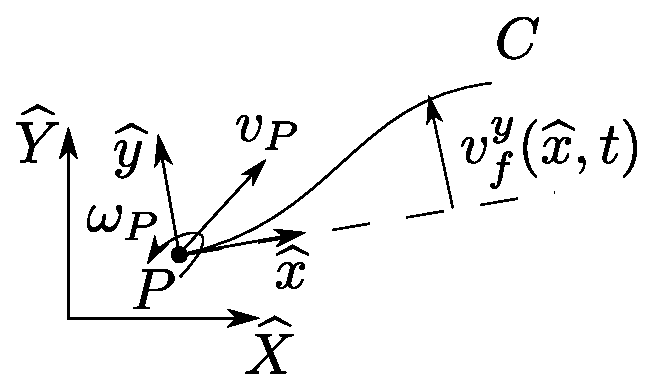
\includegraphics[width=0.5\textwidth]{part_4/pHfmd/beam.eps} 
	\caption{Floating beam. The rigid motion is located at point P}
	\label{fig:beam}
\end{figure}

A thin planar flexible beam is considered as mechanical model. The dependence of the canonical momenta on the deformation field is neglected. This hypothesis usually applies in the floating frame formulation, since the deformations are small. $P$ is placed at the origin of the local frame $P:\{x=0\}$, while $C$ is the ending point of the beam $C:\{x=L\}$ (see Fig. \ref{fig:beam}). The beam has length $L$, Young modulus $E$, density $\rho$, cross section $A$ and second moment of area $I$. The model in strong form for a flexible beam is then written compactly as 
\begin{equation}
\label{eq:EB_str_phdae}
\begin{aligned}
\begin{bmatrix}
\bm{I} & \bm{0} \\
\bm{0} & \mathcal{M} \\
\end{bmatrix}
\begin{pmatrix}
\dot{\bm{q}} \\
\dot{\bm{p}} \\
\end{pmatrix}
&= \begin{bmatrix}
\bm{0} & {\mathcal{J}}_{qe} \\
-{\mathcal{J}}_{qe}^* & {\mathcal{J}}_e \\
\end{bmatrix}
\begin{pmatrix}
\partial_{\bm{q}} H \\
\bm{p}  \\
\end{pmatrix} + 
\begin{bmatrix}
\bm{0} \\
{\mathcal{B}}_r \\
\end{bmatrix} \bm{u}_\partial, \\
\bm{u}_\partial &= {\mathcal{B}}_{\partial} \bm{p}, \\
\bm{y}_\partial &= {\mathcal{C}}_{\partial} \bm{p},
\end{aligned}
\end{equation}
The state and boundary vectors are expressed as
\begin{align*}
\bm{q} &= [^i\bm{r}_P, \; \bm{R}_{\text{v}}, \; \bm{u}_f]^\top \\
\bm{p} &= [v_P^x, \; v_P^y, \; \omega_P^z, \; v_f^x, \; v_f^y, \; n_x, \; m_{x}]^\top, \\
\bm{u}_\partial &=  [F_{P}^x, \; F_{P}^y, \; T_{P}^z, \; F_{C}^x, \; F_{C}^y, \; T_{C}^z]^\top, \\
\bm{y}_\partial &=  [v_{P}^x, \; v_{P}^y, \; \omega_{P}^z, \; v_{C}^x, \; v_{C}^y, \; \omega_{C}^z]^\top.
\end{align*}
The state contains the generalized coordinates $\bm{q}$, the linear and angular velocity $v_P^x, \; v_P^y, \; \omega_P^z$ at point $P$, the deformation velocity $ v_f^x, \; v_f^y$ and the traction and bending stress $n_x, \; m_{x}$. The boundary input contains the forces and torques acting at the extremities of the beam, while the boundary output contains the corresponding conjugated variables (velocities and angular velocities).
The deformation field has to be constrained, to prevent rigid movement (see Remark \ref{rmk:MB_dirich}). The appropriate selection of the boundary condition for the deformation field is an unavoidable problem that depends on the particular case under consideration.  Depending on the application, cantilever or simply supported boundary conditions may be considered
\begin{equation*}
\text{Cantilever}
\begin{cases}
u_f^x(x=0) = 0, \\
u_f^y(x=0) = 0, \\
\partial_x u_f^y(x=0) = 0, \\
\end{cases} \qquad 
\text{Simply supported}
\begin{cases}
u_f^x(x=0) = 0, \\
u_f^y(x=0) = 0, \\
u_f^y(x=L) = 0. \\
\end{cases}
\end{equation*}
Partitioning the $\bm{p}$ vector into rigid $\bm{p}_r = [v_P^x, \ v_P^y, \ \omega_P^z]^\top$ and flexible part $\bm{p}_f = [v_f^x, \ v_f^y, \ n_x, \ m_{x}]^\top$, the mass operator is then structured as follows
\begin{equation}
\label{eq:EB_M}
{\mathcal{M}} = 
\left[ \begin{array}{c:c}
{\mathcal{M}}_{rr} & {\mathcal{M}}_{rf} \\
\hdashline
{\mathcal{M}}_{fr} & {\mathcal{M}}_{ff} \\
\end{array} \right] = 
\left[ \begin{array}{ccc:cccc}
m & 0 & 0 & \mathcal{I}_\rho^L & 0 & 0 & 0 \\
0 & m & s^x & 0 & \mathcal{I}_\rho^L & 0 & 0 \\
0 & s^x & J^{zz} & 0 & \mathcal{I}_{\rho x}^{L} & 0 & 0 \\
\hdashline 
(\mathcal{I}_\rho^{L})^* & 0 & 0 & \rho A & 0 & 0 & 0  \\
0 & (\mathcal{I}_\rho^{L})^* & (\mathcal{I}_{\rho x}^{L})^* & 0 & \rho A & 0 & 0  \\
0 & 0 & 0 & 0 & 0 & (EA)^{-1} & 0 \\
0 & 0 & 0 & 0 & 0 & 0 & (EI)^{-1} \\
\end{array} \right],
\end{equation}
where  $s^x = \int_{0}^{L} \rho A x \d{x}$ is the static moment, $J^{zz} = \int_{0}^{L} \rho A x^2 \d{x}$ is the moment of inertia, $\mathcal{I}_\rho^L := \int_{0}^L \rho A (\cdot) \d{x}, \; \mathcal{I}_{\rho x}^L := \int_{0}^L \rho A x (\cdot) \d{x}$. Differently from standard Lagrangian formulations, the mass operator includes the coefficients $(EA)^{-1}$ and $(EI)^{-1}$. These coefficients represent the compliance of the beam and appear in the mass operator to include the deformation energy
	\begin{equation*}
	H_{\text{def}} = \frac{1}{2}\int_{0}^L \frac{1}{EA} n_x^2 + \frac{1}{EI} m_x^2  \d\Omega.
	\end{equation*}
The interconnection operator is found by adapting the cross product to the planar case:
\begin{equation}
\label{eq:EB_J}
\mathcal{J}_{e}(\bm{e}) = 
\left[ \begin{array}{c:c}
{\mathcal{J}}_{rr} & {\mathcal{J}}_{rf} \\
\hdashline
{\mathcal{J}}_{fr} & {\mathcal{J}}_{ff} \\
\end{array} \right] = 
\left[ \begin{array}{ccc:cccc}
0 & 0 & +\widehat{p}_t^y      & 0 & 0 & 0 & 0 \\
0 & 0 & -\widehat{p}_t^x     & 0 & 0 & 0 & 0 \\
-\widehat{p}_t^y & +\widehat{p}_t^x & 0 & -\mathcal{I}_{p_f^y}^{L} & +\mathcal{I}_{p_f^x}^{L} & 0 & 0 \\
\hdashline 
0 & 0 & +(\mathcal{I}_{p_f^y}^{L})^* & 0 & 0 & \partial_x & 0  \\
0 & 0 & -(\mathcal{I}_{p_f^x}^{L})^* & 0 & 0 & 0 & -\partial_{xx} \\
0 & 0 & 0 & \partial_{x} & 0 & 0 & 0 \\
0 & 0 & 0 & 0 & \partial_{xx} & 0 & 0 \\
\end{array} \right],
\end{equation}
where $\widehat{p}_t^x, \widehat{p}_t^y$ are the modified canonical momenta components (see \eqref{eq:mod_momenta}) and 
$$\mathcal{I}_{p_f^x}^{L} := \int_{0}^{L} \left\{2 p_f^x + \rho A v_f^x \right\} (\cdot) \d{x}, \qquad \mathcal{I}_{p_f^y}^{L} := \int_{0}^{L} \left\{2 p_f^y + \rho A v_f^y \right\} (\cdot) \d{x}.$$ 

The control operator reads
\begin{equation}
{\mathcal{B}}_r = \begin{bmatrix}
\bm{I}_{3\times 3} & \bm\tau_{CP}^\top \\
\bm{0}_{4\times 3} & \bm{0}_{4\times 3} \\
\end{bmatrix} \qquad \text{with} \quad
\bm\tau_{CP} = \begin{bmatrix}
1 & 0 & 0 \\
0 & 1 & L \\
0 & 0 & 1 \\
\end{bmatrix}.
\end{equation}

The discretization procedure detailed in \secref{sec:MB_discr} is extended to this case, considering that the differential operators are 
\[
{\mathcal{J}}_{\Div} = \begin{bmatrix}
\partial_x & 0 \\
0 & -\partial_{xx} \\
\end{bmatrix}, \qquad 
\mathcal{J}_{\Grad} = \begin{bmatrix}
\partial_x & 0 \\
0 & \partial_{xx} \\
\end{bmatrix}.
\]
These two operators play the same role as $\Div, \; \Grad$. The 2 PDEs associated to the first and second line of $\mathcal{J}_{\Div}$ are integrated by parts once and twice respectively, so that the boundary forces and momenta are naturally included in the discretized system as inputs. The finite-dimensional system then reads
\begin{equation}
\label{eq:EB_sys}
\begin{aligned}
\begin{bmatrix}
\mathbf{I} & \mathbf{0} & \mathbf{0} \\
\mathbf{0} & \mathbf{M}_{rr} & \mathbf{M}_{rf}\\ 
\mathbf{0} & \mathbf{M}_{fr} & \mathbf{M}_{ff}\\
\end{bmatrix} 
\begin{pmatrix}
\dot{\mathbf{q}} \\ 
\dot{\mathbf{p}}_{r} \\ 
\dot{\mathbf{p}}_{f} \\ 
\end{pmatrix} &= 
\begin{bmatrix}
\mathbf{0} & \mathbf{J}_{qr}(\mathbf{q}) & \mathbf{J}_{qf} \\
\mathbf{J}_{rq}(\mathbf{q}) & \mathbf{J}_{rr}(\mathbf{p}) & \mathbf{J}_{rf}(\mathbf{p})\\ 
\mathbf{J}_{fq} & \mathbf{J}_{fr}(\mathbf{p}) & \mathbf{J}_{ff}\\
\end{bmatrix}  
\begin{pmatrix}
\partial_{\mathbf{q}} H \\
{\mathbf{p}}_{r} \\ 
{\mathbf{p}}_{f} \\ 
\end{pmatrix} + 
\begin{bmatrix}
\mathbf{0} \\
\mathbf{B}_{r} \\ 
\mathbf{B}_{f} \\ 
\end{bmatrix}
\mathbf{u}_\partial, \\
\mathbf{y}_\partial &= \begin{bmatrix}
\mathbf{0} \ & \mathbf{B}_{r}^\top & \mathbf{B}_{f}^\top  
\end{bmatrix} \begin{pmatrix}
\mathbf{q} \\
{\mathbf{p}}_{r} \\ 
{\mathbf{p}}_{f} \\ 
\end{pmatrix},
\end{aligned}
\end{equation}
Matrix $\mathbf{B}_{r} = [\mathbf{I}_{3\times 3} \quad \bm\tau_{CP}^\top]$ accounts for the effect of boundary forces on the rigid part. Matrix $\mathbf{B}_{f}$  is the result of the integration by parts
\begin{align*}
\mathbf{B}_{f} = \begin{bmatrix}
\mathbf{0}_{n_f^{vx} \times 3} & \bm{\phi}_{v_f^x}(L) & \mathbf{0}_{n_f^{vx}} & \mathbf{0}_{n_f^{vx}} \\
\mathbf{0}_{n_f^{vy} \times 3} & \mathbf{0}_{n_f^{vy}} & \bm{\phi}_{v_f^y}(L) & \partial_x \bm{\phi}_{v_f^y}(L) \\
\mathbf{0}_{n_f^{\sigma x} \times 3} & \mathbf{0}_{n_f^{\sigma x}} & \mathbf{0}_{n_f^{\sigma x}} & \mathbf{0}_{n_f^{\sigma x}} \\
\mathbf{0}_{n_f^{\sigma y} \times 3} & \mathbf{0}_{n_f^{\sigma y}} & \mathbf{0}_{n_f^{\sigma y}} & \mathbf{0}_{n_f^{\sigma y}} \\
\end{bmatrix},
\end{align*}
where $\bm{\phi}_{v_f^x}, \ \bm{\phi}_{v_f^y}$ are the shape functions for ${v}_f^x, {v}_f^y$ and $\bm{\phi}_{v_f^x}$. Fields ${v}_f^x, {v}_f^y, n_x, m_x$ are approximated using $n_f^{vx}, n_f^{vy}, n_f^{\sigma x}, n_f^{\sigma y}$ degrees of freedom respectively. System \eqref{eq:EB_sys} can be rewritten compactly as
\begin{equation}
\label{eq:beam_discr}
\begin{aligned}
\mathbf{E} \dot{\mathbf{e}} &= \mathbf{J}(\mathbf{e}) \mathbf{z}(\mathbf{e}) + \mathbf{B}_\partial \mathbf{u}_\partial, \vspace{2mm} \\
\mathbf{y}_\partial &= \mathbf{B}_\partial^{\top}  \mathbf{z}. \\
\end{aligned}
\end{equation}
This model describes the motion of a flexible floating beam that undergoes small deformations. 

\section{Multibody systems in pH form}
\label{sec:MB_pH}
In Sections \secref{sec:pH_fd}, and \secref{sec:MB_discr}, the pH formulation of a single flexible floating body in infinite- and finite-dimensional form was presented. The construction of a multibody system is accomplished by exploiting the modularity of the port-Hamiltonian framework. Each element of the system is interconnected to the others by means of classical pH interconnections.

\subsection{Interconnections of pHDAE systems}
Consider two generic pHDAE systems of the form
\begin{equation}
\begin{cases}
\mathbf{E}_i \dot{\mathbf{e}}_i = \mathbf{J}_i \mathbf{z}_i(\mathbf{e}_i) + \mathbf{B}_i^{\text{int}} \mathbf{u}_i^{\text{int}} + \mathbf{B}_i^{\text{ext}} \mathbf{u}_i^{\text{ext}}  \vspace{2mm} \\
\mathbf{y}_i^{\text{int}} = \mathbf{B}_i^{\text{int} \top}  \mathbf{z}_i \\
\mathbf{y}_i^{\text{ext}} = \mathbf{B}_i^{\text{ext} \top}  \mathbf{z}_i \\
\end{cases} \qquad \forall i = 1, 2.
\end{equation}
where $\partial_{\mathbf{e}_i} {H_i} = \mathbf{E}_i^\top \mathbf{z}_i$. Systems of this kind arise from the discretization of formulation \eqref{eq:MFD_pHDAE}. The interconnection uses the internal control $\mathbf{u}_i^{\text{int}}$. An interconnection is said to be power preserving if and only if the following holds
\begin{equation} \label{eq:int_balance}
\langle \mathbf{u}_1^{\text{int}}, \; \mathbf{y}_1^{\text{int}} \rangle + \langle \mathbf{u}_2^{\text{int}}, \; \mathbf{y}_2^{\text{int}} \rangle = 0,
\end{equation}

which expresses that the power going out from one system flows in the other in a lossless manner. Two interconnections are of interest when coupling system: the gyrator and transformer interconnections.

\paragraph{Gyrator interconnection}
The gyrator interconnection reads
\begin{equation*}
\mathbf{u}_1^{\text{int}} = -\mathbf{C} \mathbf{y}_2^{\text{int}}, \qquad
\mathbf{u}_2^{\text{int}} = \mathbf{C}^\top \mathbf{y}_1^{\text{int}}.
\end{equation*}
This interconnection verifies \eqref{eq:int_balance} and provides the system
\begin{align*}
\begin{bmatrix}
\mathbf{E}_1 & \mathbf{0} \\ \mathbf{0} & \mathbf{E}_2 \\
\end{bmatrix}
\begin{pmatrix}
\dot{\mathbf{e}}_1 \\ \dot{\mathbf{e}}_2 \\
\end{pmatrix} &= 
\begin{bmatrix}
\mathbf{J}_1 & -\mathbf{B}_1^{\text{int}} \mathbf{C} \mathbf{B}_2^{\text{int} \top} \\ 
\mathbf{B}_2^{\text{int}} \mathbf{C} \mathbf{B}_1^{\text{int} \top}  & \mathbf{J}_2 \\
\end{bmatrix}
\begin{pmatrix}
\mathbf{z}_1 \\ 
\mathbf{z}_2 \\
\end{pmatrix}+ 
\begin{bmatrix}
\mathbf{B}_1^{\text{ext}} & \mathbf{0} \\ \mathbf{0} & \mathbf{B}_2^{\text{ext}} \\
\end{bmatrix} 
\begin{pmatrix}
\mathbf{u}_1^{\text{ext}} \\ \mathbf{u}_2^{\text{ext}} \\
\end{pmatrix}  \\
\begin{pmatrix}
\mathbf{y}_1^{\text{ext}} \\ \mathbf{y}_2^{\text{ext}} \\
\end{pmatrix}  &= \begin{bmatrix}
\mathbf{B}_1^{\text{ext} \top} & \mathbf{0} \\
\mathbf{0} & \mathbf{B}_2^{\text{ext} \top} \\
\end{bmatrix} \begin{pmatrix}
\mathbf{z}_1 \\ 
\mathbf{z}_2 \\
\end{pmatrix}.
\end{align*}

\paragraph{Transformer interconnection}
The transformer interconnection reads
\begin{equation*}
\mathbf{u}_1^{\text{int}} = -\mathbf{C} \mathbf{u}_2^{\text{int}}, \qquad
\mathbf{y}_2^{\text{int}} = \mathbf{C}^\top \mathbf{y}_1^{\text{int}}.
\end{equation*}
Again, this interconnection verifies \eqref{eq:int_balance}. After the interconnection the final system is differential algebraic:
\begin{align*}
\begin{bmatrix}
\mathbf{E}_1 & \mathbf{0} & \mathbf{0} \\ 
\mathbf{0} & \mathbf{E}_2 & \mathbf{0} \\
\mathbf{0} & \mathbf{0} & \mathbf{0} \\
\end{bmatrix}
\begin{pmatrix}
\dot{\mathbf{e}}_1 \\ \dot{\mathbf{e}}_2 \\ \dot{\bm{\lambda}} \\
\end{pmatrix} &= 
\begin{bmatrix}
\mathbf{J}_1 & \mathbf{0} & -\mathbf{B}_1^{\text{int}} \mathbf{C} \\ 
\mathbf{0} & \mathbf{J}_2 & \mathbf{B}_2^{\text{int}} \\
\mathbf{C}^\top \mathbf{B}_1^{\text{int} \top} & - \mathbf{B}_2^{\text{int} \top} & \mathbf{0} \\
\end{bmatrix}
\begin{pmatrix}
\mathbf{z}_1 \\ 
\mathbf{z}_2 \\
\bm{\lambda} \\
\end{pmatrix}+ 
\begin{bmatrix}
\mathbf{B}_1^{\text{ext}} & \mathbf{0} \\
\mathbf{0} & \mathbf{B}_2^{\text{ext}} \\
\mathbf{0} & \mathbf{0} \\
\end{bmatrix} 
\begin{pmatrix}
\mathbf{u}_1^{\text{ext}} \\ 
\mathbf{u}_2^{\text{ext}} \\
\end{pmatrix} \\
\begin{pmatrix}
\mathbf{y}_1^{\text{ext}} \\ \mathbf{y}_2^{\text{ext}} \\
\end{pmatrix}  &= \begin{bmatrix}
\mathbf{B}_1^{\text{ext} \top} & \mathbf{0} & \mathbf{0} \\
\mathbf{0} & \mathbf{B}_2^{\text{ext} \top} & \mathbf{0} \\
\end{bmatrix} \begin{pmatrix}
\mathbf{z}_1 \\ 
\mathbf{z}_2 \\
\bm{\lambda} \\
\end{pmatrix}.
\end{align*}



\subsection{Application to multibody systems of beams}
\label{sec:int_beams}
Once a discretized system is obtained, lossless joints can be modeled as a transformer interconnection. A common example is a revolute joint between two beams. Considering discretization \eqref{eq:beam_discr}, the boundary control input $\mathbf{u}_{\partial, i}$ may be split into interconnection variables $\mathbf{u}_i^{\text{int}}$ and external variables  $\mathbf{u}_i^{\text{ext}}$, i.e. $\mathbf{u}_{\partial, i} = [\mathbf{u}_i^{\text{int}}; \ \mathbf{u}_i^{\text{ext}}]$. The same splitting applies to the output. In this case the interconnection variables are
\begin{equation*}
\begin{aligned}
\mathbf{u}_1^{\text{int}} &= [F^x_{C_1}, \, F^y_{C_1}]^\top := \mathbf{F}_{C_1}, \\
\mathbf{u}_2^{\text{int}} &= [F^x_{P_2}, \, F^y_{P_2}]^\top := \mathbf{F}_{P_2},
\end{aligned} \qquad
\begin{aligned}
\mathbf{y}_1^{\text{int}} &= [v^x_{C_1}, \, v^y_{C_1}]^\top := \mathbf{v}_{C_1}, \\
\mathbf{y}_2^{\text{int}} &= [v^x_{P_2}, \, v^y_{P_2}]^\top := \mathbf{v}_{P_2}.
\end{aligned}
\end{equation*}
The interconnection matrix is the relative rotation matrix between the two local frames
\begin{equation}
\mathbf{R}(\theta) = \begin{bmatrix}
\cos(\theta) & - \sin(\theta) \\
\sin(\theta) & \cos(\theta) \\
\end{bmatrix}, \qquad 
\begin{aligned}
\theta(t) &= \theta(0) + \int_{0}^t (\omega^z_{P_2} - \omega^z_{P_1}) \d{\tau}.
\end{aligned}
\end{equation}

\begin{figure}[t]
	\centering
	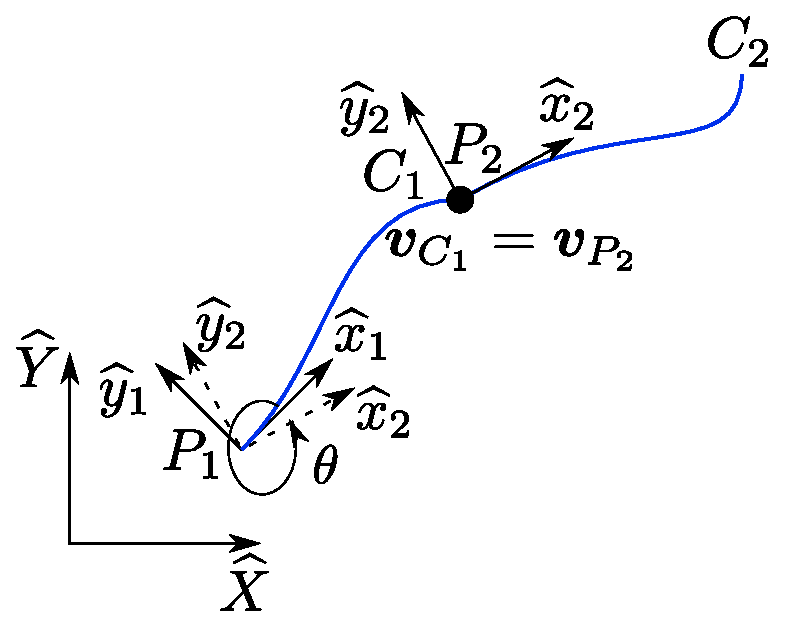
\includegraphics[width=0.45\textwidth]{part_4/pHfmd/beam_int.eps} 
	
	\caption{Two beams interconnected by an hinge }
	\label{fig:beam_int}
\end{figure}

The transformer interconnection
\begin{equation}
\label{eq:int_hinge}
\mathbf{u}_1^{\text{int}} = -\mathbf{R}(\theta) \mathbf{u}_2^{\text{int}}, \qquad
\mathbf{y}_2^{\text{int}} = \mathbf{R}(\theta)^\top \mathbf{y}_1^{\text{int}},
\end{equation}
imposes the constraints on the velocity level and gives rise to a quasi-linear index 2 pHDAE:

\begin{equation}
\label{eq:int_beams}
\begin{aligned}
\begin{bmatrix}
\mathbf{E}_1 & \mathbf{0} & \mathbf{0} \\ 
\mathbf{0} & \mathbf{E}_2 & \mathbf{0} \\
\mathbf{0} & \mathbf{0} & \mathbf{0} \\
\end{bmatrix}
\begin{pmatrix}
\dot{\mathbf{e}}_1 \\ \dot{\mathbf{e}}_2 \\ \dot{\bm{\lambda}} \\
\end{pmatrix} &= 
\begin{bmatrix}
\mathbf{J}_1(\mathbf{e}_1) & \mathbf{0} & -\mathbf{B}_1^{\text{int}} \mathbf{R} \\ 
\mathbf{0} & \mathbf{J}_2(\mathbf{e}_2) & \mathbf{B}_2^{\text{int}} \\
\mathbf{R}^\top \mathbf{B}_1^{\text{int} \top} & - \mathbf{B}_2^{\text{int} \top} & \mathbf{0} \\
\end{bmatrix}
\begin{pmatrix}
\mathbf{z}_1  \\ 
\mathbf{z}_2  \\ 
\bm{\lambda} \\
\end{pmatrix}+ 
\begin{bmatrix}
\mathbf{B}_{\partial 1}^{\text{ext}} & \mathbf{0} \\
\mathbf{0} & \mathbf{B}_{\partial 2}^{\text{ext}} \\
\mathbf{0} & \mathbf{0} \\
\end{bmatrix} 
\begin{pmatrix}
\mathbf{u}_1^{\text{ext}} \\ 
\mathbf{u}_2^{\text{ext}} \\
\end{pmatrix}, \\
\begin{pmatrix}
\mathbf{y}_1^{\text{ext}} \\ \mathbf{y}_2^{\text{ext}} \\
\end{pmatrix}  &= \begin{bmatrix}
\mathbf{B}_{\partial 1}^{\text{ext} \top} & \mathbf{0} & \mathbf{0} \\
\mathbf{0} & \mathbf{B}_{\partial 2}^{\text{ext} \top} & \mathbf{0} \\
\end{bmatrix} \begin{pmatrix}
\mathbf{z}_1  \\ 
\mathbf{z}_2  \\ 
\bm{\lambda} \\
\end{pmatrix}.
\end{aligned}
\end{equation}

\begin{remark}
	The constraints  are imposed at a velocity level to preserve the pH structure. It is well-known that a drift appears in this case. For linear systems it is possible to use the \textit{Gear-Gupta-Leimkuhler} formulation to preserve the pH structure and enforce the constraints directly on the positions \cite{scholz2019}. In the non-linear case, stabilization technique may be introduced to avoid drifting phenomena \cite{bauchau2008review,laulusa2008review}. 
\end{remark}

The same result can be obtained by using a pHDAE system and a gyrator interconnection. To illustrate this, consider the pHDAE obtained by interchanging the role of output and input of the second system $\mathbf{u}_2^{\text{int}} \leftrightarrow \mathbf{y}_2^{\text{int}}$. The output then plays the role of a Lagrange multiplier. The input $\mathbf{u}_2^{\text{int}}$ is now considered as Lagrange multiplier ${\bm{\lambda}}_2$ and the output $\mathbf{y}_2^{\text{int}}$ plays the role of $\mathbf{u}_2^{\text{int}}$. The discretized system assumes the following differential-algebraic structure
\begin{equation}
\begin{aligned}
\begin{bmatrix}
\mathbf{E}_2 & \mathbf{0} \\
\mathbf{0} & \mathbf{0} \\
\end{bmatrix} \begin{pmatrix}
\dot{\mathbf{e}}_2 \\
\dot{\bm{\lambda}}_2 \\
\end{pmatrix}
&= \begin{bmatrix}
\mathbf{J}_2(\mathbf{e}_2) & \mathbf{B}_2^{\text{int}} \\
-\mathbf{B}_2^{\text{int} \top} & \mathbf{0}\\
\end{bmatrix} \begin{pmatrix}
\mathbf{z}_2 \\
{\bm{\lambda}}_2
\end{pmatrix} 
+ \begin{bmatrix}
\mathbf{0} \\
\mathbf{I}
\end{bmatrix} \mathbf{u}_2^{\text{int}} + \begin{bmatrix}
\mathbf{B}_2^{\text{ext}} \\
\mathbf{0} \\
\end{bmatrix} \mathbf{u}_2^{\text{ext}},  \vspace{2mm} \\
\mathbf{y}_2^{\text{int}} &= \begin{bmatrix}
\mathbf{0} & \mathbf{I}
\end{bmatrix}\begin{pmatrix}
\mathbf{z}_2 \\
{\bm{\lambda}}_2
\end{pmatrix}, \\
\mathbf{y}_2^{\text{ext}} &= \begin{bmatrix}
\mathbf{B}_2^{\text{ext} \top} & \mathbf{0}
\end{bmatrix}\begin{pmatrix}
\mathbf{z}_2 \\
{\bm{\lambda}}_2
\end{pmatrix}.
\end{aligned}
\end{equation}
This system is improper, since the input appears in the algebraic part. Now, a gyrator interconnection is used to model the hinged joint
\begin{equation}
\label{eq:int_hinge_DAE}
\mathbf{u}_1^{\text{int}} = -\mathbf{R}(\theta) \mathbf{y}_2^{\text{int}}, \qquad
\mathbf{u}_2^{\text{int}} = \mathbf{R}(\theta)^\top \mathbf{y}_1^{\text{int}}.
\end{equation}
The resulting differential-algebraic system is exactly \eqref{eq:int_beams}, which is proper. The equivalence between the two representations is represented in Fig. \ref{fig:beam_int_block}. This approach allows the modular construction of systems of arbitrary complexity. Other kinds of lossless joints (prismatic, spherical) can be modeled by appropriate interconnections. The system can then be simulated by using specific DAE solvers \cite{brenan1995dae}. 

\begin{figure}[t]
	\centering
	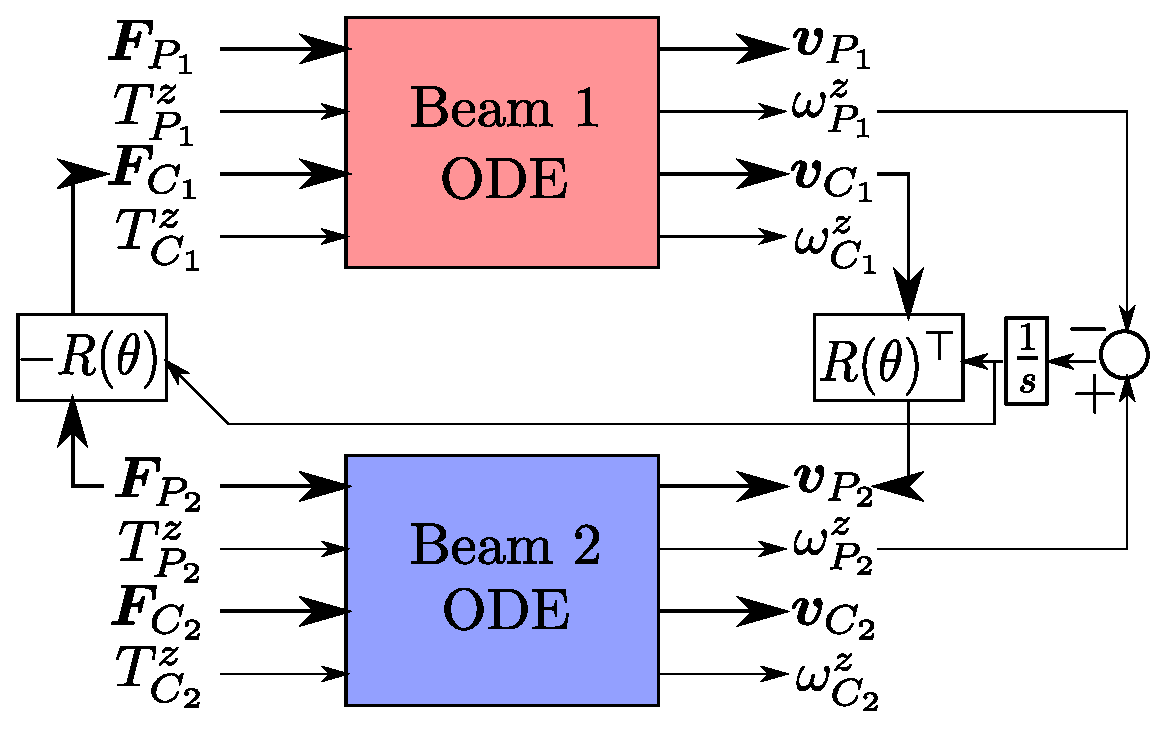
\includegraphics[height=0.16\textheight]{part_4/pHfmd/block_hinged_beam.eps} \hspace{.5cm}
	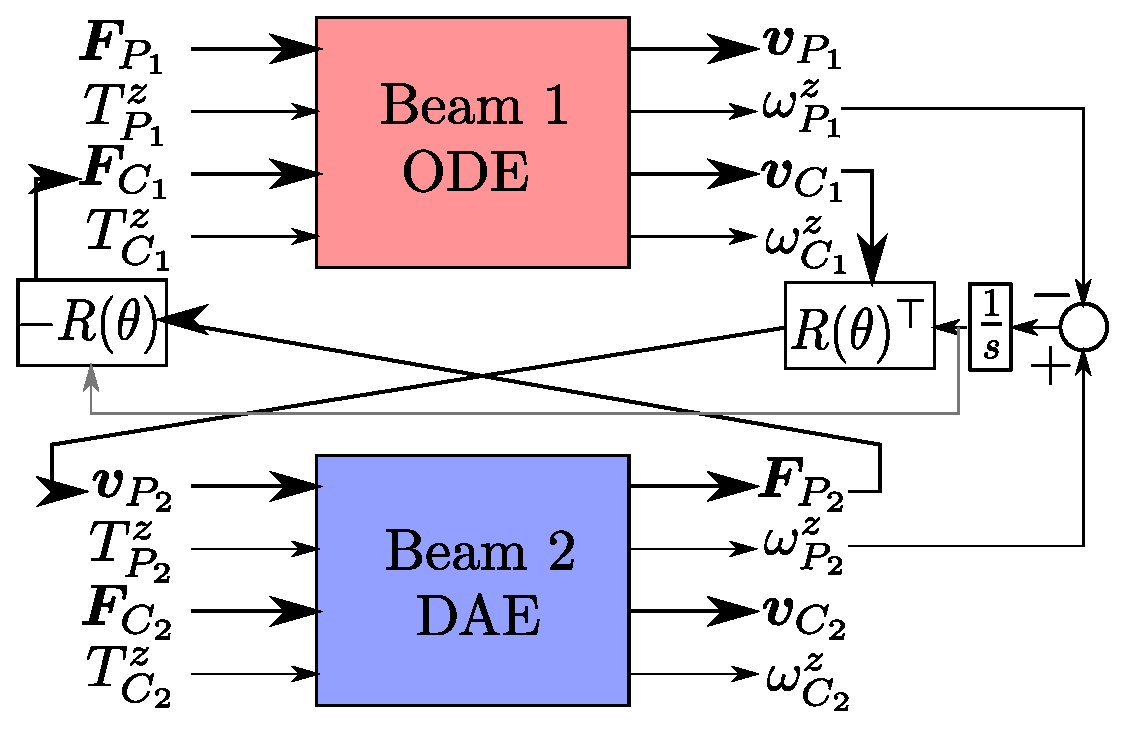
\includegraphics[height=0.16\textheight]{part_4/pHfmd/block_hinged_beam_DAE.eps} 	
	\caption{Block diagrams representing the transformer interconnection \eqref{eq:int_hinge} (left) and the equivalent gyrator interconnection \eqref{eq:int_hinge_DAE} (right)}
	\label{fig:beam_int_block}
\end{figure}

\subsection{The linear case: substructuring and model reduction}
If the angular velocities and the relative orientations are small then the system may be linearized about a particular geometrical configuration. Omitting the partition related to the generalized coordinates $\mathbf{q}$ and partitioning the system into rigid and flexible dynamics, the resulting equations are then expressed as 
\begin{equation}
\label{eq:mbd_linear}
\begin{bmatrix}
\mathbf{M}_{rr} & \mathbf{M}_{rf} & \mathbf{0} \\ 
\mathbf{M}_{fr} & \mathbf{M}_{ff} & \mathbf{0} \\
\mathbf{0} & \mathbf{0} & \mathbf{0} \\
\end{bmatrix}
\begin{pmatrix}
\dot{\mathbf{p}}_r \\ \dot{\mathbf{p}}_f \\ \dot{\bm{\lambda}} \\ 
\end{pmatrix} = 
\begin{bmatrix}
\mathbf{0} & \mathbf{0} & \mathbf{G}_r^\top \\ 
\mathbf{0} & \mathbf{J}_{ff} & \mathbf{G}_f^\top \\ 
-\mathbf{G}_r & -\mathbf{G}_f & \mathbf{0} \\
\end{bmatrix}
\begin{pmatrix}
\mathbf{p}_r \\ \mathbf{p}_f \\ {\bm{\lambda}} \\ 
\end{pmatrix} + 
\begin{bmatrix}
\mathbf{B}_r \\ \mathbf{B}_f \\ \mathbf{0} \\
\end{bmatrix}\mathbf{u}.
\end{equation}
The Hamiltonian is now a quadratic function of the state variables $H = \frac{1}{2} \mathbf{p}^\top\mathbf{M}\mathbf{p}$ \cite{beattie2018linear}.
The modular construction of complex multi-body systems is then analogous to a substructuring technique \cite{klerk2008}, where the velocities and forces are linked at the interconnection points. Such system can be reduced using Krylov subspace method directly on the DAE formulation \cite{egger2018}. The basic idea relies on the construction of a subspace $\mathbf{V}_f^{\text{red}}$ for the vector $\mathbf{p}_f$ such that $\mathbf{p}_f \approx \mathbf{V}_f^{\text{red}} \mathbf{p}_f^{\text{red}}$. The reduced system then reads
\begin{equation}
\begin{bmatrix}
\mathbf{M}_{rr} & \mathbf{M}_{rf}^{\text{red}} & \mathbf{0} \\ 
\mathbf{M}_{fr}^{\text{red}} & \mathbf{M}_{ff}^{\text{red}} & \mathbf{0} \\
\mathbf{0} & \mathbf{0} & \mathbf{0} \\
\end{bmatrix}
\begin{pmatrix}
\dot{\mathbf{p}}_r \\ \dot{\mathbf{p}}_f^{\text{red}} \\ \dot{\bm{\lambda}} \\ 
\end{pmatrix} = 
\begin{bmatrix}
\mathbf{0} & \mathbf{0} & \mathbf{G}_r^\top \\ 
\mathbf{0} & \mathbf{J}_{ff}^{\text{red}} & \mathbf{G}_f^{\text{red} \top} \\ 
-\mathbf{G}_r & -\mathbf{G}_f^{\text{red}} & \mathbf{0} \\
\end{bmatrix}
\begin{pmatrix}
\mathbf{p}_r \\ \mathbf{p}_f^{\text{red}} \\ {\bm{\lambda}} \\ 
\end{pmatrix} + 
\begin{bmatrix}
\mathbf{B}_r \\ \mathbf{B}_f^{\text{red}} \\ \mathbf{0} \\
\end{bmatrix}\mathbf{u},
\end{equation}
where the second row has been pre-multiplied by $\mathbf{V}_f^{\text{red} \top}$. Alternatively, a null space matrix can employed to eliminate the Lagrange multiplier and preserve the port-Hamiltonian structure. Consider the pHDAE \eqref{eq:mbd_linear}, where the differential and algebraic parts are explicitly separated

\begin{equation}
\begin{aligned}
\mathbf{M} \dot{\mathbf{p}} &=  \mathbf{J}\mathbf{p} + \mathbf{G}^\top \bm{\lambda} + \mathbf{B}\mathbf{u}, \\ 
\mathbf{0} &= \mathbf{G}\mathbf{p},
\end{aligned}
\end{equation}
and consider a matrix $\mathbf{P}$ that satisfies 
\[
\mathrm{range}\{\mathbf{P}\} = \mathrm{null}\{\mathbf{G}\}.
\]
Then, the range of $\mathbf{P}$ automatically satisfies the constraints. Considering the transformation $\widehat{\mathbf{p}} = \mathbf{P} \mathbf{p}$ and pre-multiplying the system by $\mathbf{P}^\top$ an equivalent ODE is obtained
\[
\widehat{\mathbf{M}} \ \dot{\widehat{\mathbf{p}}} =  \widehat{\mathbf{J}} \ \widehat{\mathbf{p}} + \widehat{\mathbf{B}} \ \mathbf{u},
\]
with $\widehat{\mathbf{M}} = \mathbf{P}^\top \mathbf{M} \mathbf{P}, \; \widehat{\mathbf{J}} = \mathbf{P}^\top \mathbf{J} \mathbf{P}, \; \widehat{\mathbf{B}} = \mathbf{P}^\top \mathbf{B}$. The computation of $\mathbf{P}$ can be performed by QR decomposition of matrix $\mathbf{G}$ \cite{leyendecker2008nullspace}. A pH system in standard form is then obtained considering the variable change $\widehat{\mathbf{x}} = \widehat{\mathbf{M}} \widehat{\mathbf{p}}$
\[ \dot{\widehat{\mathbf{x}}} =  \widehat{\mathbf{J}} \widehat{\mathbf{Q}}\ \widehat{\mathbf{x}} + \widehat{\mathbf{B}}  \mathbf{u}, \qquad \widehat{\mathbf{Q}}:= \widehat{\mathbf{M}}^{-1}.
\] 
Once an equivalent ODE formulation is obtained the concepts and ideas presented in \cite{chaturantabut2016} can be used to reduce the flexible dynamics.


\section{Conclusion}
A port-Hamiltonian formulation for the flexible multibody dynamics has been discussed. The equations of motions proposed in the paper  are obtained by direct manipulation of pre-existing results, unveiling the Hamiltonian structure of the floating frame of reference formulation. \\
\indent The discretization procedure uses a mixed finite element method, hence, the stress distribution is available without any post-processing. This is a valuable characteristic of this framework, as the stress distribution is the most important variable for preliminary analysis of mechanical components. \\
\indent This approach allows treating different models and their interconnections in a common framework. This formulation works with any kind of rigid joints and could be easily extended for any kind of flexible joints. The construction of multibody system becomes completely modular and well suited for control applications. \\
\indent In the following chapter, the proposed formulation is tested for some benchmark problems.

